% Classe do Documento ---------------------------------------------------------
\documentclass[12pt]{report}

% Pacotes ---------------------------------------------------------------------
\usepackage{eulervm}
\usepackage{fontspec}
  \setmainfont{Alegreya}
  [
    Path          = fonts/alegreya/,
    Extension     = .ttf,
    UprightFont   = *-Regular,
    BoldFont      = *-Bold,
    ItalicFont    = *-Italic
  ]
\usepackage{polyglossia}
  \setdefaultlanguage[variant = brazilian]{portuguese}
\usepackage{graphicx}
	\graphicspath{{./figs/}}
\usepackage[labelfont = bf, font = small]{caption}
\usepackage[a5paper]{geometry}
\usepackage{fancybox}
\usepackage{fancyhdr}
\usepackage{booktabs}
  \renewcommand{\arraystretch}{1.5}
\usepackage{mathtools, amsthm, amssymb, amscd}
  \makeatletter
    \renewcommand*\env@matrix[1][*\c@MaxMatrixCols c]{%
      \hskip -\arraycolsep
      \let\@ifnextchar\new@ifnextchar
      \array{#1}}
  \makeatother
\usepackage{systeme}
\usepackage{cancel}
\usepackage{esvect}
\usepackage{stackrel}
\usepackage{array}
  \setcounter{MaxMatrixCols}{20}
\usepackage{xcolor}
\usepackage{hyperref} 																											
  \hypersetup
  {
    colorlinks  = true,
    linkcolor   = blue,
    citecolor   = blue,
    filecolor   = blue,
    urlcolor    = blue,
    pdfproducer = {LaTeX},
    pdfcreator  = {XeLaTeX},
    pdfauthor   = {Ícaro Vidal Freire},
    pdfsubject  = {Aulas do Professor Jabes}, 
    pdfkeywords = {programação linear, linear programming, algebra linear}
 }
\usepackage{tikz}
\usepackage{tikz-cd}

% Configurações ---------------------------------------------------------------

% Teoremas 
\newtheorem{teorema}{Teorema}
\newtheorem{exemplo}{Exemplo}
\newtheorem{obs}{Observação}

% Operadores
\DeclareMathOperator{\Min}{Min}

% Novos Comandos
\newcommand{\custoGeral}[1]{c_{1}x_{1} + c_{2}x_{x} + \ldots + c_{n}x_{n} }
\newcommand{\linhaSistema}[1]{a_{#11}x_{1} + a_{#12}x_{2} + \ldots + a_{#11}x_{n}}
\newcommand{\inversaA}{\left(A^{I}\right)^{-1}}
\newcommand{\setaEntra}[1]{
  \ensuremath{\stackrel{\textcolor{red}{\downarrow}}{x_{#1}}}
}
\newcommand{\setaSai}[1]{
  \ensuremath{\hspace{-0.55cm}\textcolor{red}{\leftarrow}\, x_{#1}}
}

\newcommand{\circulo}[1]{
  \tikz[baseline=(char.base)]
  {
    \node[shape = circle, draw, inner sep = 2pt, dashed, draw = blue] (char) {$#1$};
  }
}

% Cabeçalho de todo o texto ---------------------------------------------------
\renewcommand{\headrulewidth}{2pt}
\renewcommand{\footrulewidth}{0.7pt}

% Configurando o Título -------------------------------------------------------
\title
{
  \textbf{Programação Linear}  \\
  {\large (Notas de Aula)}\\
  \vspace{1.5cm}
  {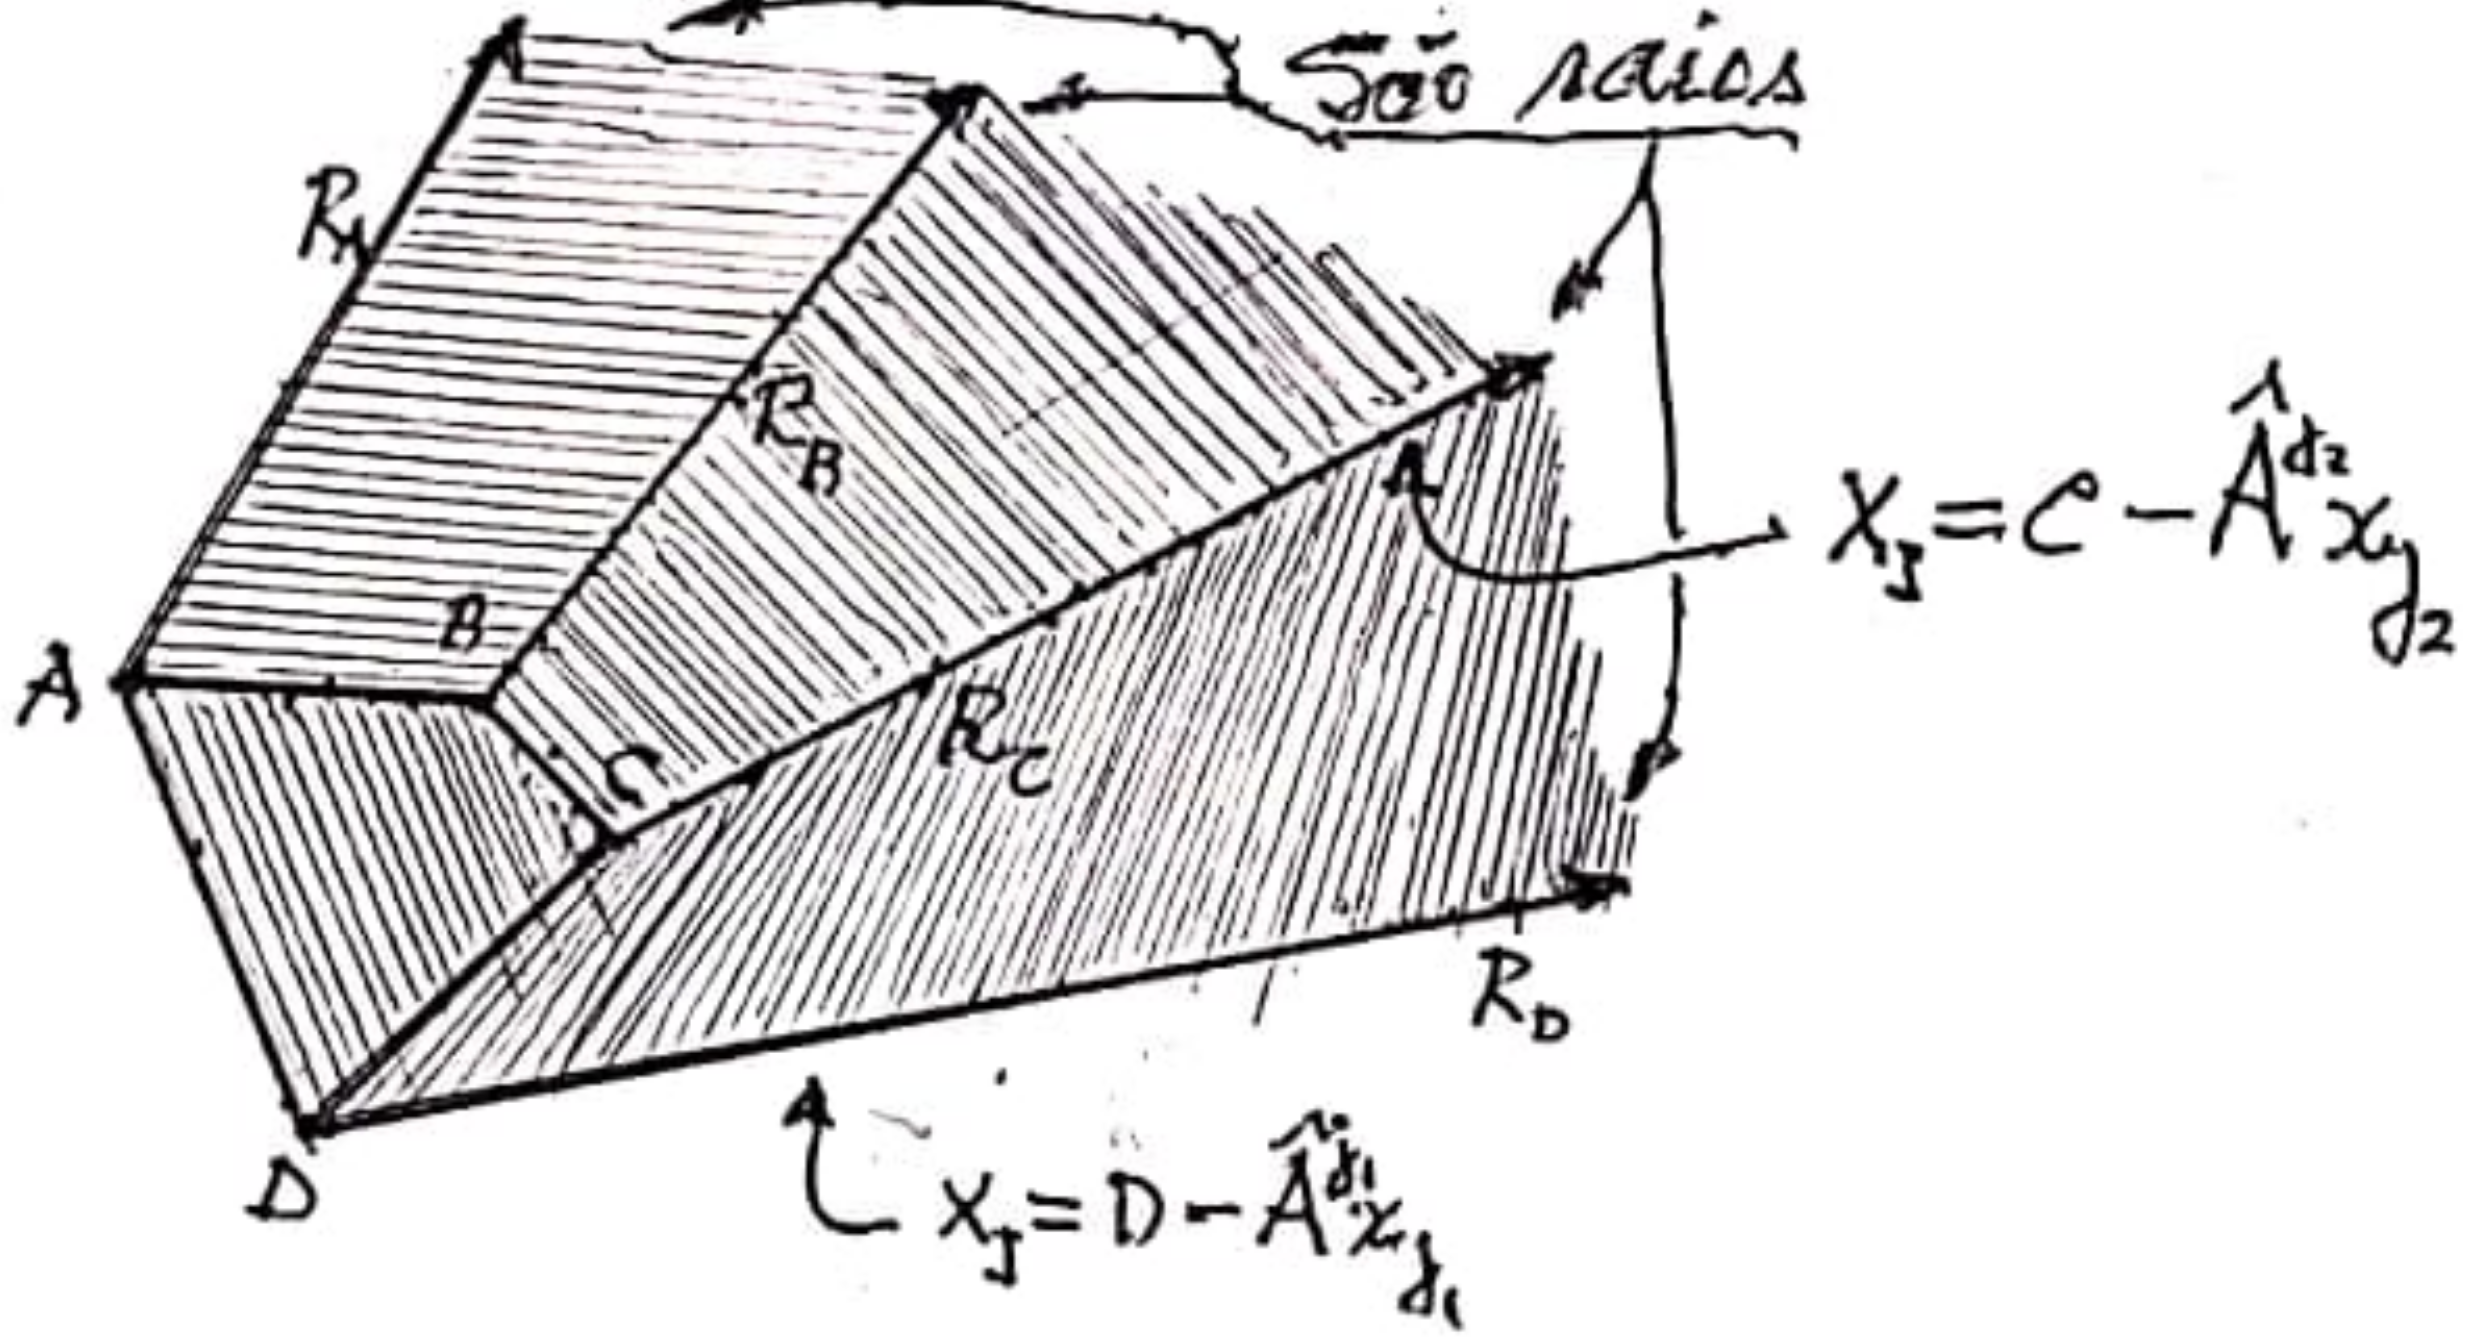
\includegraphics[width = 0.5\linewidth]{belo_desenho.png}}
}
\author{Jabes F. A. Silva}
\date{2021}

% Início do Documento =========================================================
\begin{document}
%
  \pagestyle{empty} % tira o cabeçalho da primeira página
%
  \maketitle
%
  \tableofcontents
  \cleardoublepage
%
  \pagestyle{fancy}
  \fancyhf{}
  \fancyhead[LE,RO]{\leftmark}
  \fancyhead[RE,LO]{}
  \fancyfoot[CE,CO]{\thepage}
  \fancyfoot[LE,RO]{}
%
% Incluindo as aulas ----------------------------------------------------------
  %==============================================================================
% Programação Linear
% 25/08/2021
%==============================================================================

\chapter{Programação Linear}

\section{Discussão da Solução Ótima} %-----------------------------------------

Antes de entrarmos na discussão da solução ótima faremos alguns comentários sobre
o \textbf{Método Simplex}.

O Método Simplex faz uso do algorítimo \textbf{Simplex Duas Fases}.
A Fase I é requerida quando após se acrescentar as variáveis de folga e de excesso
às inequações, isto é, passar o problema à forma padrão, não se vislumbra uma
solução básica factível de pronto.
O objetivo da Fase I é obter uma solução básica factível inicial.
A Fase II é o algorítimo propriamente dito, que para começar as iterações requer
uma solução básica factível inicial.
Os problemas cujas restrições são inequações do tipo ``menor ou igual'', e lembrando
que o vetor $ b $ é sempre positivo, têm sempre uma solução básica factível
inicial.
Nos outros casos, em geral, não tem uma solução básica factível inicial, logo,
necessitam de proceder a Fase I.

Para discussão da solução ótima, suporemos que se tem uma solução básica factível
inicial.
Logo, vamos utilizar a Fase II.

Tanto na Fase I, como na Fase II, a cada iteração verifica-se se a solução básica
atual é ótima.
Se é ótima, fim.
Se não é ótima, se vai para o critério de escolha da variável não básica que deve 
ser a candidata para entrar na base.
Escolhida a variável não básica candidata a entrar na base vem o critério da 
variável básica que sairá da base.

Pode ocorrer empate, tanto para a escolha da variável entrante, como para escolha
da que vai sair.
Ditas essas coisas em linhas gerais, vamos aos detalhes.

Voltemos ao sistema de equações,

\begin{align*}
  \min \quad        & z = c_I \inversaA b + \left[c_J - c_I \inversaA A^{J}\right] x_J\\
  \text{s.a.} \quad & x_I + \inversaA A^{J} x_J = \inversaA b \\
                    & x_I, x_J \geq 0
\end{align*}

Na Função Objetivo a parte variável é a segunda parcela do segundo membro,

\[
  \left[ c_J - c_I \inversaA A^{J} \right]  x_J
\]

Suponha que a solução básica atual é ótima.
Isto significa que o valor de $ z $, que é $ c_I \inversaA b $, não tem mais 
como diminuir, ou seja, se algum $ x_j $ (variável não básica) aumentar de valor,
o valor de $ z $ aumentará.
Isto implica que o coeficiente $ \widehat{c}_j $ de $ x_j $ é positivo.
Por outro lado, se todos os $ \widehat{c}_j > 0 $, qualquer variável $ x_j $
que aumentar de valor fará o valor de $ z $ também aumentar, logo, a solução 
atual é ótima.

Conclusão:

\begin{center}
\fbox
{
  \begin{minipage}{0.7\linewidth}
    A solução básica atual é ótima e única se, e somente se, $ \widehat{c}_j > 0 $,
    $ \forall j \in J $.
  \end{minipage}
}
\end{center}

Se a solução básica atual é ótima e algum $ \widehat{c}_j = 0 $, haverá infinitas 
soluções ótimas, pois para cada valor positivo que $ x_j $ assumir corresponderá 
a novos valores das variáveis básicas, mas o valor de $ z $ permanece o mesmo, 
ou seja, $ c_I \inversaA b $, pois $ \widehat{c}_j x_j = 0 $.
Para saber os valores das variáveis básicas para cada valor positivo assumido
por $ x_j $, observe a equação de bloqueio:

\[
  x_I + \widehat{A}^j x_j = \widehat{b}
\]

Agora cabe uma pergunta: \textit{Neste caso há outra solução básica ótima?}
Mais uma vez a resposta é dada pela equação de bloqueio.

Se algum $ \widehat{a}_ij > 0 $, haverá outra solução básica ótima, pois a 
variável básica da linha $ i $ irá para zero quando $ x_j $ aumentar de valor.
Caso haja mais de um $ \widehat{a}_ij > 0 $, as variáveis básicas das respectivas
linhas irão para zero.
Mas, se uma variável atingiu o valor zero, o $ x_j $ não pode mais aumentar de 
valor, caso contrário, a variável básica torna-se-á negativa.
Logo, $ x_j $ será bloqueado quando a primeira variável básica atingir o valor
zero.
O valor de $ x_j $ que faz a variável básica $ x_{B_i} = 0 $ é dado por:

\[
  \frac{\widehat{b}_i}{\widehat{a}_{ij}}  
\]

Assim, se houver mais de uma variável básica indo para zero, deve se escolher
aquela que primeiro atingir zero.
Para isso, calcula-se:

\[
  \min_{i}  
  \left\{\, 
    \frac
    {
      \widehat{b}_i
    }
    {
      \widehat{a}_{ij}
    }; 
    \quad 
    \widehat{a}_{ij} > 0 
  \,\right\}
\]

\begin{obs}
  Se duas ou mais variáveis básicas atingirem zero simultaneamente, estamos 
  diante de uma solução básica degenerada.
  Mas, só uma delas sai da base e $ x_j $ entra no lugar da que saiu.
\end{obs}

O cáculo iterativo para se chegar a nova solução básica é transformar a coluna
$ \widehat{A}^j $ na coluna da matriz identidade que está com a variável básica
que está saindo da base.
Se $ x_{B_i} $ é a variável básica que está saindo da base, o primeiro cálculo
a ser feito é dividir toda linha $ i $ por $ \widehat{a}_{ij} $.
A partir daí, por meio de operações elementares sobre as linhas, é transformar
em zero o $ \widehat{c}_j $ e todos os $ \widehat{a}_{kj} $, com $ k \in I $ e 
$ k \neq i $.
Feito isto, obteve-se a nova solução básica.
Agora, volta-se ao teste de otimalidade.

\section{Montagem do Quadro Simplex} %-----------------------------------------

Toda a discussão sobre a solução ótima e pivoteamento foram realizadas com o P.L.
na forma:

\begin{align*}
  \min        \quad & z = c_I \inversaA b + \left[c_J - c_I \inversaA A^J \right] x_J \\
  \text{s.a.} \quad & x_I + \inversaA A^J x_J = \inversaA b \\
                    & x_I, x_J \geq 0
\end{align*}

Para montagem do quadro, toda expressão que tiver variável colocamos no primeiro
membro das equações, e as constantes, no segundo.
Mas, para manter a discussão sem alterações, sobre o sinal de $ \widehat{c}_J $,
colocamos a F.O. na seguinte forma:

\[
  \left[c_J - c_I \inversaA A^J \right] x_J - z = -c_I \inversaA b
\]

E o quadro do Simplex é o seguinte:

\begin{table}[!htbp]
  \centering
  \begin{tabular}{c|ccc|c}
    Min         & $x_I$        & $x_J$                       &  $z$  & \\ \hline
    Var. Bás.   & $0$          & $c_J - c_I \inversaA A^{J}$ & $-1$  & $-c_I \inversaA b$\\ \hline
    $x_I$       & $\mathbb{I}$ & $\inversaA A^J$             & $0$   & $\inversaA b$ \\ \hline
                &              & $x_I, x_J \geq 0$           &       &
  \end{tabular}
\end{table}

Ou fazendo uso da notação simplificada:

\begin{table}[!htbp]
  \centering
  \begin{tabular}{c|ccc|c}
    Min       & $x_I$        & $x_J$           & $z$  & \\ \hline
    Var. Bás. & $0$          & $\widehat{c}_J$ & $-1$ & $-c_I \inversaA b$ \\ \hline
    $x_I$     & $\mathbb{I}$ & $\widehat{A}^J$ & $0$  & $\widehat{b}$ \\ \hline
              &              & $x_I, x_J$      &      &
  \end{tabular}
\end{table}

Na prática, na primeira linha, as variáveis são dispostas na ordem crescente dos
índices; e, na última linha, não colocamos.

Os procedimentos e discussões sobre a solução ótima são os mesmso tanto para a 
Fase I, como para a Fase II.

Vejamos um exemplo que não requer a Fase I.

\begin{exemplo}
  Resolva o P.L. abaixo:
  \begin{align*}
    \min        \quad & z = -3 x_1 + 5 x_2 - 2 x_3 \\
    \text{s.a.} \quad & 
                        \begin{aligned}[t]
                          2 x_1 + 2 x_2 + 4 x_3 &\leq 12 \\
                          - x_1 + 3 x_2 + 2 x_3 &\leq 6  \\
                          2 x_1 + 4 x_2 -   x_3 &\leq 4
                        \end{aligned}\\
                      & x_1, x_2, x_3 \geq 0.
  \end{align*}
\end{exemplo}

Primeiro passa o problema para forma padrão, acrescentando-se as variáveis de 
folga.

\begin{align*}
  \min        \quad & z = -3 x_1 + 5 x_2 - 2 x_3 \\
  \text{s.a.} \quad & 
                      \begin{aligned}[t]
                        2 x_1 + 2 x_2 + 4 x_3 + x_4 \phantom{+ x_5 + x_6} &= 12 \\
                        - x_1 + 3 x_2 + 2 x_3 \phantom{+ x_4} + x_5 \phantom{+ x_6}&= 6  \\
                        2 x_1 + 4 x_2 -   x_3 \phantom{+ x_4 + x_5} + x_6 &= 4
                      \end{aligned}\\
                    & x_1, x_2, x_3, x_4, x_5 \geq 0.
\end{align*}

Note que há uma solução básica factível inicial: 
\begin{itemize}
  \item \textbf{Variáveis Básicas:} $ x = 12, x_5 = 6 \text{ e } x = 4 $;
  \item \textbf{Variáveis não Básicas:} $ x_1 = x_2 = x_3 = 0$;
  \item \textbf{Valor de F.O.}: $ z = 0 $.
\end{itemize}

Montando o quadro Simplex:

\begin{table}[!htbp]
  \centering
  \begin{tabular}{c|ccccccc|c}
    Min             & $\setaEntra{1}$   & $x_2$ & $x_3$ & $x_4$ & $x_5$ & $x_6$ & $z$  &      \\ \hline
    Var. Bás.       & $-3$              & $5$   & $-2$  & $0$   & $0$   & $0$   & $-1$ & $0$  \\ \hline           
    $x_4$           & $ 2$              & $2$   & $4$   & $1$   & $0$   & $0$   & $0$  & $12$ \\
    $x_5$           & $-1$              & $3$   & $2$   & $0$   & $1$   & $0$   & $0$  & $6$  \\
    $\setaSai{6}$   & $\circulo{2}$     & $4$   & $-1$  & $0$   & $0$   & $1$   & $0$  & $4$
  \end{tabular}
\end{table}

Neste caso, em que as inequações são todos do tipo ``$\leq$'', o quadro sempre está
preparado, istó é, pronto para discussão se a solução  básica atual é ótima ou
não.

Há dois $\widehat{c} < 0$, o que indica que a solução básica atual não é ótima 
($\widehat{c}_7 = -3$ e $\widehat{c}_3 = -2$).
O mais negativo corresponde à variável não básica que deve ser a candidata a 
entrar na base.
Logo, $ x_1 $ é a candidata a entrar  na base.
Agora, examinaremos o $ \widehat{A}^{1} $.

\[
  \widehat{A}^{1} = 
    \begin{bmatrix}
      2 \\
      -1 \\
      2
    \end{bmatrix}
\]

Como há elementos positivos, há outra solução básica factível que melhora a F.O.
($\widehat{a}_{11} = 2$ e $\widehat{a}_{31} = 2$).

A equação de bloqueio é 
\[
  \begin{bmatrix}
    x_4 \\
    x_5 \\
    x_6
  \end{bmatrix}  
  +
  \begin{bmatrix}
    2 \\
    -1\\
    2
  \end{bmatrix}
  = 
  \begin{bmatrix}
    12 \\
    6 \\
    4
  \end{bmatrix},
\]
 e o cálculo prático para se saber que variável  básica sai da base é 
 \[
   \Min_{i} \left\{ \frac{\widehat{b}_i}{\widehat{a}_{ij}}; \;\; \widehat{a}_{ij} > 0 \right\}
 \]

 Assim, tem-se o seguinte:
 \[
   \Min\left\{\frac{12}{2}, \frac{4}{2}\right\}  = \frac{4}{2} = 2.
 \]

 Significa que $ x_6 $ deve sair da base, e $ x_1 $ entra na base com valor 2.
 
 Observe: se $ x_1 = 2 $, então $ x_6 = 0, x_4 = 8 \text{ e } x_5 = 8 $.

 A coluna $ \widehat{A}^{1} $ deve ser transformada na coluna 
 \[
   \begin{bmatrix} 
    0 \\ 
    0 \\ 
    1 
   \end{bmatrix} 
\] 
que é a atual coluna de $ x_6 $.

O novo quadro é:

\begin{table}[!htbp]
  \centering
  \begin{tabular}{c|ccccccc|c}
    Min           & $x_1$ & $x_2$ & $\setaEntra{3}$ & $x_4$ & $x_5$ & $x_6$ & $z$  &     \\ \hline
    Var. Bás.     & $0$   & $11$  & $-7/2$          & $0$   & $0$   & $3/2$ & $-1$ & $6$ \\ \hline
    $\setaSai{4}$ & $0$   & $-2$  & $\circulo{5}$   & $1$   & $0$   & $-1$  & $0$  & $8$ \\
    $x_5$         & $0$   & $5$   & $3/2$           & $0$   & $1$   & $1/2$ & $0$  & $8$ \\
    $x_1$         & $1$   & $2$   & $-1/2$          & $0$   & $0$   & $1/2$ & $0$  & $2$ 
  \end{tabular}
\end{table}

A solução básica atual não é ótima: $ \widehat{c}_3 = -7/2 $.
Único negativo, logo, $ x_3 $ é camdidato a entrar na base.

O elemento do encontro da coluna da variável que entra com a linha da variável 
que sai é chamado \textbf{pivô}.
Ele é que será transformado em ``1'' e todos os cálculos são realizados por meio 
dele.

Da \textbf{Equação de Bloqueio} 
\[
  \begin{bmatrix}
    x_4 \\
    x_5 \\
    x_1
  \end{bmatrix}  
  + \begin{bmatrix}
    5    \\
    3/2  \\
    -1/2 \\
  \end{bmatrix}
  = 
  \begin{bmatrix}
    8 \\
    8 \\
    2
  \end{bmatrix}
\]
se retira o cálculo prático, do qual se obtém duas informações:
\begin{enumerate}
  \item[(i)] com que valor $ x_3 $ \textbf{entra};
  \item[(ii)] e que variável \textbf{sai} da base.
\end{enumerate}

Como
\[
  Min\left\{\frac{8}{5}, \frac{8}{3/2}\right\}  = \frac{8}{5},
\]
logo, $x_4$ sai da base.

\begin{table*}[!htbp]
  \centering
  \begin{tabular}{c|ccccccc|c}
    Min       & $x_1$ & $x_2$  & $x_3$ & $x_4$   & $x_5$ & $x_6$  & $z$  &        \\ \hline
    Var. Bás. & $0$   & $48/5$ & $0$   & $7/10$  & $0$   & $4/5$  & $-1$ & $58/5$ \\ \hline 
    $x_3$     & $0$   & $-2/5$ & $1$   & $1/5$   & $0$   & $-1/5$ & $0$  & $8/5$  \\
    $x_5$     & $0$   & $28/5$ & $0$   & $-3/10$ & $1$   & $4/5$  & $0$  & $28/5$ \\
    $x_1$     & $1$   & $9/5$  & $0$   & $1/10$  & $0$   & $2/5$  & $0$  & $14/5$ 
  \end{tabular}
\end{table*}

Todos os $ \widehat{c}_J > 0 $, logo a solução básica atual é ótima e única.

\begin{itemize}
  \item $ \widehat{c}_2 = 48/5, \widehat{c}_4 = 7/10 \;\text{ e }\; \widehat{c}_6 = 4/5 $
  \item o valor ótimo de $ z $ é $ -58/5 $
  \item variáveis básicas: $ x_3 = 8/5, x_5 = 28/5 \;\text{ e }\; x_1 = 14/5 $
  \item variáveis não básicas: $ x_2 = x_4 = x_6 = 0 $
\end{itemize}

\section{Fase I} %-------------------------------------------------------------


  %%==============================================================================
% Programação Linear II
% 04/08/2021
%==============================================================================

\chapter{Programação Linear II}

\section{Solução Básica} %=====================================================

Seja $ A $ uma matriz $ m \times n $ de \textit{rank} $ m $ e considere o 
sistema $ Ax = b $ de equações lineares.
Como $ A $ tem \textit{rank} $ m $ é possível extrair de $ A $ $ m $ vetores
coluna linearmente independentes.
Com isto, é possível tirar os valores das $ m $ variáveis associadas a esses
$ m $ vetores colunas em função das $ n - m $ variáveis restantes.

Uma solução básica é obtida fazendo essas $ n - m $ variáveis restantes 
assumirem o valor zero.

\begin{exemplo}
  Considere o sistema 
  \[
   \systeme{3x_1-2x_2+5x_3+6x_4 = 4, 2x_1+3x_2+4x_3-2x_4=6}
  \]
\end{exemplo}

A matriz aqui é 
$
  \begin{bmatrix} 
   3 & -2 & 5 & 6 \\ 
   2 &  3 & 4 & -2
  \end{bmatrix}
$.
Claro que $ A $ tem \textit{rank} 2.
Em particular, quaisquer dois vetores coluna escolhidos em $ A $ são linearmente
independentes.
Escolhemos as colunas 2 e 3, o que significa que vamos tirar os valores das 
variáveis $ x_2 $ e $ x_3 $ em termos das variáveis $ x_1 $ e $ x_2 $.
Há diversas maneiras de se resolver, mas vamos fazer uso de inversão de matrizes,
no caso, calculando a inversa da matriz $\begin{bmatrix} -2 & 5 \\ 3 & 4\end{bmatrix}$.

A inversa\footnote{Para matrizes $ 2 \times 2 $ há uma maneira prática de se 
calcular a inversa. 
Se $ A = \begin{bmatrix} a & b \\ c & d\end{bmatrix} $, então a sua inversa é
$ \dfrac{1}{ad - bc}\begin{bmatrix} d & -b \\ -c & a\end{bmatrix} $
} é 
$
  \dfrac{-1}{23}
  \begin{bmatrix} 
    4 & -5 \\ 
   -3 & -2
  \end{bmatrix}
$.
Agora é só multiplicar todo o sistema por essa inversa.

Podemos fazer o cálculo só com as matrizes para economizar tempo, mas 
acrescentando a coluna independente, $ \begin{bmatrix} 4 \\ 6\end{bmatrix}$.

{\scriptsize
\begin{align*}
  -\frac{1}{23} 
  \begin{bmatrix} 
    4 & -5 \\ 
    &\\
   -3 & -2
  \end{bmatrix} 
  \begin{bmatrix}[cccc|c]
   3 &-2 & 5 &  6 & 4 \\
    &&&&\\
   2 & 3 & 4 & -2 & 6
  \end{bmatrix}
  &=
  -\frac{1}{23}
  \begin{bmatrix}[cccc|c]
     2 & -23 &   0 &  34 & -14 \\
     &&&&\\
   -13 &   0 & -23 & -14 & -24
  \end{bmatrix}\\ \\
  &= 
  \begin{bmatrix}[cccc|c]
   -\frac{2}{23}  & 1 & 0 & -\frac{34}{23} & \frac{14}{23} \\
                  &   &   &                &               \\
    \frac{13}{23} & 0 & 1 &  \frac{14}{23} &\frac{24}{23}
  \end{bmatrix}
\end{align*}
}

Portanto, \systeme*{x_2 = \frac{14}{23} + \frac{2}{23}x_1+\frac{34}{23}x_4, x_3 = \frac{24}{23} + \frac{13}{23}x_1+\frac{14}{23}x_4}.

Tomando $ x_1 = x_4 = 0 $, obtém-se a solução básica referente a $ x_2 $ e 
$ x_3 $:

\[
\systeme*{x_2 = \frac{14}{23}, x_3 = \frac{24}{23}}.
\]

Em Programação Linear há um adicional a mais com relação às variáveis: elas 
devem ser maiores ou iguais a zero.
É uma restrição a mais que não interfere na definição de solução básica.
Então, na linguagem  de P.L., o que se diz é que, se os valores básicos 
encontrados são maiores ou iguais a zero, diz-se que é uma 
\textbf{solução básica factível}.
Caso contrário, diz-se \textbf{solução básica infactível}.
O sistema proposto é:

\[
  Ax = b, \qquad x \geq 0.
\]

Outro detalhe importante é que uma solução básica pode ser identificada pelos
índices das variáveis que não assumirão o valor zero.
Essas são denominadas de \textbf{variáveis básicas}, e aquelas que assumirão o
valor zero são denominadas de \textbf{variáveis não básicas}.
Também são ditas que essas $ m $ variáveis básicas estão na base e as não básicas
estão fora da base.
Portanto, os índices das variáveis básicas, dizem quem é a solução básica.
Mas, para completar essa identificação é necessário saber em que linha ou 
equação está a variável básica.
Isto impõe que os índices devem estar ordenados na mesma sequência em que as
correspondentes variáveis aparecem nas linhas.
Assim, o primeiro índice deve ser da variável básica que está na primeira linha,
o segundo índice, da variável básica que está na segunda linha e assim por 
diante.
Dessa forma, defini-se um conjunto ordenados dos índices das variáveis básicas,
que será denotado por $ I $; e, um outro conjunto dos índices das variáveis não
básicas, denotado por $ J $.

No exemplo dado: $ I = \{\,2, 3\,\} $ e $ J = \{\,1. 4\,\} $.

De agora em diante, uma solução básica será identificada pelo conjunto $ I $.

\begin{exemplo}
  Dado o sistema 
  \[
   \systeme
   {
     x_1 + 5x_2 - x_3 =  5,
    3x_1 + 4x_2 + x_4 = 12,
    2x_1 +  x_2 - x_5 =  4
   }
  \]
  com $ x_1, x_2, x_3, x_4, x_5 \geq 0 $ e I = \{\,2, 4, 1\,\}.
\end{exemplo}


Significa que foram tirados  os valores das variáveis $ x_1 $, $ x_2 $ e $ x_3 $,
mas que a ordem em que aparecem na solução final é que $ x_2 $ está na primeira
linha, $ x_4 $ está na segunda e $ x_1 $ está na terceira linha.
Veja abaixo:

\[
  \systeme
  {
   x_2 - \frac{2}{9}x_3 + \frac{1}{9}x_5  = \frac{2}{3},
   \frac{5}{9}x_3 + x_4 + \frac{11}{9}x_5 = \frac{13}{3},
   x_1 + \frac{1}{9}x_3 - \frac{5}{9}x_5  = \frac{5}{3}
  }
\]

A solução básica é: $ x_2 = \frac{2}{3} $, $ x_4 = \frac{13}{3} $ e 
$ x_4 = \frac{5}{3} $.
As variáveis não básicas: $ x_3 = x_5 = 0 $.

A matriz dos vetores coluna extraídos da matriz \\

\[ 
  A = 
  \begin{bmatrix} 
   1 & 5 & -1 & 0 &  0 \\
   3 & 4 &  0 & 1 &  0 \\
   2 & 1 &  0 & 0 & -1
  \end{bmatrix} 
  \qquad
  \text{ é }
  \qquad
  \begin{bmatrix}
   5 & 0 & 1 \\
   4 & 1 & 3 \\
   1 & 0 & 2
  \end{bmatrix}.
\]

Observe a ordem das colunas.
A primeira coluna é a do $ x_2 $; a segunda coluna é a do $ x_4 $ e a terceira
coluna é a do $ x_1 $.
Assim, quando multiplicar a matriz estendida do sistema pela inversa de 
$
  \begin{bmatrix}
   5 & 0 & 1 \\
   4 & 1 & 3 \\
   1 & 0 & 2
  \end{bmatrix}
$,
as colunas da matriz identidade aparecerá na mesma ordem, isto é, a primeira
coluna da matriz identidade estará na coluna do $ x_2 $, a segunda, na coluna do
$ x_4 $ e a terceira, na coluna do $ x_1 $.

Mostraremos que acontece exatamente isso.

\begin{align*}
  \begin{bmatrix}[ccc|ccc]
   5 & 0 & 1 & 1 & 0 & 0 \\
   4 & 1 & 3 & 0 & 1 & 0 \\
   1 & 0 & 2 & 0 & 0 & 1
  \end{bmatrix}
  &\approx
  \begin{bmatrix}[ccc|ccc]
   1 & -1 & -2 &  1 & -1 & 0 \\
   0 &  5 & 11 & -4 &  5 & 0 \\
   0 &  1 &  4 & -1 &  1 & 1 
  \end{bmatrix} \\
  &\approx
  \begin{bmatrix}[ccc|ccc]
   1 & 0 &  2 &  0 & 0 &   1 \\
   0 & 9 &  0 & -5 & 9 & -11 \\
   0 & 0 & -9 &  1 & 0 &  -5
  \end{bmatrix} \\
  &\approx 
  \begin{bmatrix}[ccc|ccc]
   9 & 0 & 0 &  2 & 0 &  -1 \\
   0 & 9 & 0 & -5 & 9 & -11 \\
   0 & 0 & 9 &  1 & 0 &  -5
  \end{bmatrix} \\
  &\approx 
  \begin{bmatrix}[ccc|ccc]
   1 & 0 & 0 &  2/9 & 0 &  -1/9 \\
   0 & 1 & 0 & -5/9 & 1 & -11/9 \\
   0 & 0 & 1 &  1/9 & 0 &  -5/9
  \end{bmatrix}
\end{align*}

Portanto a matriz inversa é 
$
  \begin{bmatrix}
    2/9 & 0 &  -1/9 \\
   -5/9 & 1 & -11/9 \\
    1/9 & 0 &  -5/9
  \end{bmatrix}
$.

Agora, vamos multiplicar essa matriz inversa pela matriz estendida dos 
coeficientes das variáveis, isto é, $ \begin{bmatrix} A & b \end{bmatrix} $.

{\scriptsize
\[
  \begin{bmatrix}
    2/9 & 0 &  -1/9 \\
   -5/9 & 1 & -11/9 \\
    1/9 & 0 &  -5/9
  \end{bmatrix}
  \begin{bmatrix}[ccccc|c]
   1 & 5 & -1 & 0 &  0 &  5 \\
   3 & 4 &  0 & 1 &  0 & 12 \\
   2 & 1 &  0 & 0 & -1 &  4 
  \end{bmatrix}
  =
  \begin{bmatrix}[ccccc|c]
   0 & 1 & -2/9 & 0 &  1/9 &  2/3 \\
   0 & 0 &  5/9 & 1 & 11/9 & 11/3 \\
   1 & 0 &  1/9 & 0 & -5/9 &  5/3
  \end{bmatrix}
\]
}

Note que a primeira coluna da matriz identidade é a segunda coluna da matriz
acima; que a coluna de $ x_2 $.
Analogamente para as outras colunas.

A leitura das linhas, por exemplo, da segunda linha, é:
\[
  \frac{5}{9}x_3 + x_4 + \frac{11}{9}x_5 = \frac{11}{3}.
\]

Leitura dos valores básicos, lê-se direto só as variáveis básicas e seus 
respectivos valores.
\[
  x_2 = \frac{2}{3}, \quad x_4 = \frac{11}{3} \quad \text{e} \quad x_1 = \frac{5}{3}.
\]





\section{Discussão da Solução Ótima} %=========================================

Considere o P.L. $ \text{Min. } z = cx $ sujeito à $ Ax = b $, $ x \geq 0 $.

As hipóteses são as de sempre: $ A $ é uma matriz $ m \times n $ de \textit{rank}
$ m $.

O ponto de partida é que se tenha uma solução básica factível inicial.

O que vamos apresentar é o \textbf{Algorítimo Simplex Duas Fases}.
A \textit{Fase I} é aplicada quando não se tem uma solução básica factível 
inicial.
A \textit{Fase II}, que é o algorítimo propriamente dito, precisa de usa solução
básica factível inicial para começar as iterações.
Em cada solução básica factível deve se proceder a discussão sobre se essa 
solução é ótima ou não.
Se não é ótima, vem a discussão se há outra solução básica que melhore o valor
da F.O.
Se existe, fazem-se os cálculos, procedimento para se passar à nova solução 
básica.
Se não há outra solução básica, diz-se que o problema tem solução ótima 
ilimitada.

\subsection{Fase I - Procedimentos} %------------------------------------------

\begin{enumerate}
	\item Abandone temporariamente a F.O. original do problema.
 \item Na parte das restrições, acrescente uma variável artificial em cada 
  equação em que não tenha uma variável básica factível.
  Essas variáveis devem ser maiores ou iguais a zero.
 \item Crie uma F.O. artificial a ser minimizada, que é constituída pela soma 
  das variáveis artificiais que foram introduzidas nas restrições.
 \item Monte o quado do simplex.
 \item Prepare o quadro, isto é, transformar os coeficientes das variáveis 
  básicas, que estão na F.O., em zero.
 \item Comece a discussão da solução ótima.
\end{enumerate}

\begin{exemplo}
  Considere o P.L.
  \[
   \begin{array}{rrcl}
    \textrm{Max}  & z = 4x_1 + 3x_2 &      &    \\
    \textrm{s.a.} & x_1 + 5x_2      & \geq & 5  \\
                  & 3x_1 + 4x_2     & \leq & 12 \\ 
                  &     2x_1 + x_2  & \geq & 4  \\ 
                  &     x_1, x_2    & \geq & 0  
   \end{array}
  \]
\end{exemplo}

A primeira coisa a ser feita é passar o problema para forma padrão.
Isto é feito acrescentando-se as variáveis de folga e de excesso, transformando
as desigualdades em equações.

\[
  \begin{array}{rlcl}
   \textrm{Max}  & z = 4x_1 + 3x_2 &                            &    \\
   \textrm{s.a.} & \phantom{3}x_1 +  5x_2 - x_3  \phantom{-0x_4}  \phantom{-0x_5}  & =    & 5  \\
                 &           3x_1 +  4x_2            \phantom{- 0x_3} + x_4 \phantom{- 0x_5}  & =    & 12 \\ 
                 &           2x_1 +  \phantom{0}x_2  \phantom{- 0x_3}  \phantom{+0x_4} - x_5   & =    & 4  \\ 
                 &  x_1, x_2, x_3, x_4, x_5 \geq 0                    &  &   
  \end{array}
\]

Observe que há uma solução básica inicial, mas é infactível.

$ x_3 = -5 $, $ x_4 = 12 $ e $ x_5 = -4 $ são as variáveis básicas.
$ x_1 $ e $ x_2 $ são as variáveis \textbf{não} básicas e que assumem o valor
zero.

Portanto há necessidade de proceder a \textit{Fase I}.

Há necessidade de variáveis artificiais na primeira e na terceira equações.
Tem-se:
\[
  \begin{array}{lc}
   \text{Min}  & w = x_6 + x_7  \\
   \text{s.a.} & \\
               & \sysdelim..\systeme
               {
               x_1 + 5x_2 - x_3 + x_6 = 5,
               3x_1 + 4x_2 + x_4 = 12,
               2x_1 + x_2 - x_5 + x_7 = 4
               }
  \end{array}
\]

Agora se tem uma solução básica factível, mas é artificial, ela não pertence ao
problema original.

Variáveis básicas: $ x_6 = 5 $, $ x_4 = 12 $ e $ x_7 = 4 $.

Variáveis não básicas: $ x_1 = x_2 = x_3 = x_5 = 0 $.

Valor da F.O.: $ w = 9 $.

Passando ao quadro:

\begin{table}[!h]
\centering
\caption{O quadro não está preparado}
\begin{tabular}{|c|cccccccc|c|}
  \hline
  Min         & $x_1$ & $x_2$ & $x_3$ & $x_4$ & $x_5$ & $x_6$ & $x_7$ & $x_8$ &    \\
  \hline
  Var. Bas.   &   0   &   0 &   0 &   0 &   0 &   1 &   1 &  -1 &  0 \\
  \hline
  $x_6$       &   1   &   5 &  -1 &   0 &   0 &   1 &   0 &   0 &  5 \\
  $x_4$       &   3   &   4 &   0 &   1 &   0 &   0 &   0 &   0 & 12 \\
  $x_7$       &   2   &   1 &   0 &   0 &  -1 &   0 &   1 &   0 &  4 \\
  \hline
\end{tabular}
\end{table}

\begin{table}[!h]
\centering
\caption{O quadro está preparado}
\begin{tabular}{|c|cccccccc|c|}
  \hline
  Min                    & $x_1$ & \textcolor{red}{$x_2$} & $x_3$ & $x_4$ & $x_5$ & $x_6$ & $x_7$ & $x_8$ &     \\
  \hline
  Var. Bas.              &   -3  &   -6                   &   1   &   0   &   1   &   0   &   0   &  -1   &  -9 \\
  \hline
  \textcolor{red}{$x_6$} &   1   &   \textcolor{red}{5}   &  -1   &   0   &   0   &   1   &   0   &   0   &   5 \\
  $x_4$                  &   3   &   4                    &   0   &   1   &   0   &   0   &   0   &   0   &  12 \\
  $x_7$                  &   2   &   1                    &   0   &   0   &  -1   &   0   &   1   &   0   &   4 \\
  \hline
\end{tabular}
\end{table}

A equação de bloqueio é:\;  $ x_{I} + \widehat{A}^{j}x_{J} = \widehat{b} $.

O cálculo prático é:\;  $ \underset{i}{\text{Min}} \left\{\,\frac{\widehat{b}_i}{\widehat{a}_{ij}} \colon \widehat{a} > 0\,\right\} $

\[
  \text{Min}\left\{\,\frac{5}{5}, \frac{12}{4}, \frac{4}{1}\,\right\} = \frac{5}{5} \Longrightarrow x_6 \text{ sai da base }
\]

Os cálculos são feitos com o objetivo de transformar a coluna do $ x_2 $ na 
coluna do $ x_6 $.
Assim, o encontro da coluna da variável que deve entrar na base com a linha da
variável básica que sai da base, $ x_6 $, é o \textcolor{red}{5}.
Este ``5'' é dito \textbf{pivô}.
 
\begin{table}[!h]
\centering
\caption{$\text{Min}\{\,\frac{1}{1/5}, \frac{8}{11/5}, \frac{3}{9/5}\,\} = \frac{3}{9/5} \Rightarrow x_7 \text{ sai da base}$}
\begin{tabular}{|c|cccccccc|c|}
  \hline
  Min                    & \textcolor{red}{$x_1$}   & $x_2$ & $x_3$ & $x_4$ & $x_5$ & $x_6$ & $x_8$ &  w  &    \\
  \hline
  Var. Bas.              &                    -9/5  & 0     & -1/5  & 0     & 1     & 6/5   & 0     & -1  & -3 \\
  \hline 
  $x_2$                  &                    1/5   &   1   &  -1/5 &     0 &   0   &   1/5 &   0   &   0 &  1 \\
  $x_4$                  &                   11/5   &   0   &   4/5 &     1 &   0   &  -4/5 &   0   &   0 &  8 \\
  \textcolor{red}{$x_7$} &   \textcolor{red}{9/5}   &   0   &  -1/5 &     0 &  -1   &  -1/5 &   1   &   0 &  3 \\
  \hline
\end{tabular}
\end{table} 
 
\begin{table}[!h]
\centering
\caption{Problema original é factível}
\begin{tabular}{|c|cccccccc|c|}
  \hline
  Min         & $x_1$ & $x_2$ & $x_3$ & $x_4$ & $x_5$ & $x_6$ & $x_7$ & $w$ &    \\
  \hline
  Var. Bas.   &   0   &   0 &   0 &   0 &   0 &   1 &   1 &  -1 &  0 \\
  \hline
  $x_2$       &   0   &   1 &  -2/9 &   0 &    1/9 &    2/9 &   -1/9 &   0 &  2/3 \\
  $x_4$       &   0   &   0 &   5/9 &   1 &   11/9 &   -5/9 &  -11/9 &   0 & 13/3 \\
  $x_1$       &   1   &   0 &   1/9 &   0 &   -5/9 &   -1/9 &    5/9 &   0 &  5/3 \\
  \hline
\end{tabular}
\end{table}

A solução básica factível atual é ótima e $ w = 0 $ indica que o problema 
original é factível. \hfill (\textbf{Fim da Fase I})

Agora se tem uma solução básica factível do problema original: $ x_2 = \frac{2}{3} $,
$ x_4 = \frac{13}{3} $ e $ x_1 = \frac{5}{3} $.
Com estes vetores, $ z = \frac{26}{3} $.

Agora é a vez de montar o quadro para \textbf{Fase II}.

Retomando a F.O. original: \newpage

\begin{table}[!h]
\centering
\caption{Quadro ainda não preparado}
\begin{tabular}{|c|cccccc|c|}
  \hline
  Min         & $x_1$ & $x_2$ & $x_3$ & $x_4$ & $x_5$ & $z$  &      \\
  \hline
  Var. Bas.   &  4    &   3   &     0 &   0   &     0 &  -1  & 0    \\
  \hline
  $x_2$       &  0    &   1   &  -2/9 &   0   &   1/9 &   0  & 2/3  \\
  $x_4$       &  0    &   0   &   5/9 &   1   &  11/9 &   0  & 13/3 \\
  $x_1$       &  1    &   0   &   1/9 &   0   &  -5/9 &   0  & 5/3  \\
  \hline
\end{tabular}
\end{table}

Falta preparar o quadro para poder fazer a discussão da solução ótima.

\begin{table}[!h]
\centering
\caption{Quadro preparado}
\begin{tabular}{|c|cccccc|c|}
  \hline
  Min                    & $x_1$ & $x_2$ & $x_3$ & $x_4$ & \textcolor{red}{$x_5$} & $z$  &       \\
  \hline
  Var. Bas.              &  0    &   0   &  -2/9 &   0   &  17/9                  &  -1  & -26/3 \\
  \hline
  $x_2$                  &  0    &   1   &  -2/9 &   0   &   1/9                  &   0  &   2/3 \\
  \textcolor{red}{$x_4$} &  0    &   0   &   5/9 &   1   &  \textcolor{red}{11/9} &   0  &  13/3 \\
  $x_1$                  &  1    &   0   &   1/9 &   0   &                   -5/9 &   0  &   5/3 \\
  \hline
\end{tabular}
\end{table}



Quadro preparado!
A solução básica factível atual não é ótima.

Fazendo da equação de bloqueio para se saber se há outra solução básica que
melhore o valor da F.O.

\begin{table}[!h]
\centering
\begin{tabular}{|c|cccccc|c|}
  \hline
  Min         & $x_1$ & $x_2$ & $x_3$ & $x_4$    & $x_5$ & $z$  &         \\
  \hline
  Var. Bas.   &  0    &   0   & -3/11 & -17/11   &     0 &  -1  & -169/11 \\
  \hline
  $x_2$       &  0    &   1   & -3/11 &  -1/11   &     0 &   0  &    3/11 \\
  $x_5$       &  0    &   0   &  5/11 &   9/11   &     1 &   0  &   39/11 \\
  $x_1$       &  1    &   0   &  4/11 &   5/11   &     0 &   0  &   40/11 \\
  \hline
\end{tabular}
\end{table}

A solução básica factível atual é ótima: 
\[ 
  x_2 = \frac{3}{11} ,  \quad x_5 = \frac{39}{11} \quad \text{ e } \quad x_1 = \frac{40}{11} .
\]
O valor ótimo de $ z $ é 

\begin{center}
  \shadowbox
  {
    $ \dfrac{169}{11} $
  }	
\end{center}

  %%==============================================================================
% Programação Linear III
% 18/08/2021
%==============================================================================

\chapter{Programação Linear III}

\section{Nomenclatura e Notação} %---------------------------------------------

Considere o problema de P.L. $ \min z = cx $ sujeito a $ Ax = b $, $ x \geq 0 $.

Aqui já foram introduzidas as variáveis de folga e de excesso.
E sobre a matriz $ A $, as hipóteses de sempre: $ A $ é $ m \times n $ de 
\textit{rank} $ m $.
O problema está na forma padrão.

O que vamos apresentar aqui são os preparativos para aplicação do 
\textbf{Algorítimo Simplex} e discussão da \textit{solução ótima}.

Como foi visto na parte \texttt{Programação Linear II}, dado o conjunto $ I $, a
solução básica fica identificada e o conjunto $ J $ também.

Suponha que se tenha uma solução básica factível $I$ de 

\begin{align*}
  \min \quad        & z = cx \\
  \text{s.a.} \quad & 
                      \begin{aligned}[t]
                        Ax &= b \\
                         x &\geq 0  
                      \end{aligned}
\end{align*}

Paralelamente, para facilitar o entendimento, expressemos o problema na forma 
escalar.

\begin{align*}
  \min \quad       & z = \custoGeral{n} \\
  \text{s.a} \quad & 
                     \begin{aligned}[t]
                       \linhaSistema{1} &= b_1 \\
                       \linhaSistema{2} &= b_2 \\
                                        &\vdots \\
                       \linhaSistema{m} &= b_m
                     \end{aligned}\\
                   & x_1, x_2, \dots, x_n \geq 0
\end{align*}

Então, $ c = \begin{bmatrix} c_1 & c_2 & \ldots & c_n \end{bmatrix} $ e 
$ x^{t} = \begin{bmatrix} x_1 & x_2 & \ldots & x_n \end{bmatrix} $.

\[
  A = \begin{bmatrix}
        a_{11} & a_{12} & \ldots & a_{1n} \\
        a_{21} & a_{22} & \ldots & a_{2n} \\
        \vdots & \vdots & \ddots & \vdots \\
        a_{m1} & a_{22} & \ldots & a_{mn} \\
      \end{bmatrix}
  \qquad
  \text{ e }
  \quad
  b = \begin{bmatrix}
        b_1 \\ 
        b_2 \\ 
        \vdots \\ 
        b_m
      \end{bmatrix}
\]

Vejamos a notação em termos dos conjuntos $ I $ e $ J $.
\[
  c = \begin{bmatrix}
        c_{I} & c_{J}
      \end{bmatrix},
  \qquad
  x = \begin{bmatrix}
        x_{I} \\
        x_{J}
      \end{bmatrix}
  \qquad
  \text{ e }
  \qquad
  A = \begin{bmatrix}
        A^{I} & A^{J}
      \end{bmatrix}
\]

Em $ c_I $ estão os coeficientes das variávis básicas na F.O. e $ c_J $ os 
coeficientes das variáveis não básicas na F.O.

Em $ x_{I} $ estão as variáveis básicas e em $ x_J $ , as não básicas.

Em $ A^{I} $ estão as colunas da matriz $ A $, correspondentes às variáveis,
cujos índices estão em $ I $ e na mesma  ordem em que aparecem em $ I $.

Em $ A^{J} $ estão as colunas da matriz $ A $ correspondentes às variáveis não
básicas, cujos índices estão em $ J $ e em geral, são colocadas em ordem 
crescente dos índices.

Como já definido em \texttt{Programação Linear II}, $ A^{I} $ é uma matriz 
$ m \times n $ \textit{inversível}, que será denotada por 
$ \left(A^I\right)^{-1} $.

Daqui em diante toda expressão que envolver a matriz $ \left( A^{I} \right)^{-1} $
será denotada com "$\^$" (chapéu).
Os conjuntos $ I $ e $ J $ desempenham papel importante nesta notação e ajudam
na discussão da solução ótima e mais adiante, na \textbf{Análise de Sensibilidade}

\begin{center}
\fbox{
  \begin{minipage}{.9\linewidth}
    \textit{Análise de Sensibilidade} é a discussão sobre o que acontece à 
    solução ótima, se algum dado inicial do problema for alterado e que 
    procedimentos efetuar.
  \end{minipage}
}
\end{center}

Vamos expressar o problema em termos de $ I $ e de $ J $.

\begin{align*}
  \min \quad         & z = \begin{bmatrix} c_I & c_j \end{bmatrix} \begin{bmatrix} x_I\\ x_J \end{bmatrix} \\
  \text{s.a.} \quad & \begin{aligned}[t]
                        \begin{bmatrix}A^I & A^J\end{bmatrix} \begin{bmatrix}x_I \\ x_J\end{bmatrix} &= b \\
                        x_I, x_j &\geq 0
                      \end{aligned}
\end{align*}

Efetuando as operações indicadas obtem-se:

\begin{align*}
  \min \quad        & z = c_Ix_I + c_Jx_J \\
  \text{s.a.} \quad &
                      \begin{aligned}
                        A^{I} x_I + A^{J}x_J &= b \\
                        x_I, x_J &\geq 0
                      \end{aligned}
\end{align*}

O método utilizado pelo Algorítimo Simplex é do \textbf{gradiente reduzido}.
O que será feito agora é multiplicar os dois membros da equação das restrições
por $ \left( A^{I} \right)^{-1} $ para encontrar os valores das variáveis 
básicas ($ x_I $) e substituí-los na F.O.

\begin{align*}
  \min \quad        & z = c_Ix_I + c_Jx_J \\
  \text{s.a.} \quad &
                      \begin{aligned}
                        \textcolor{blue}{\left( A^{I} \right)^{-1}}A^{I} x_I + \textcolor{blue}{\left( A^{I} \right)^{-1}}A^{J}x_J &= \textcolor{blue}{\left( A^{I} \right)^{-1}}b \\
                        x_I, x_J &\geq 0
                      \end{aligned}
\end{align*}

o que resulta:

\begin{align*}
  \min \quad        & z = c_Ix_I + c_Jx_J \\
  \text{s.a.} \quad &
                      \begin{aligned}
                        \mathbb{I} x_I + \left( A^{I} \right)^{-1}A^{J}x_J &= \left( A^{I} \right)^{-1}b \\
                        x_I, x_J &\geq 0
                      \end{aligned}
\end{align*}

ou ainda

\begin{align*}
  \min \quad        & z = c_Ix_I + c_Jx_J \\
  \text{s.a.} \quad &
                      \begin{aligned}
                        x_I + \left( A^{I} \right)^{-1}A^{J}x_J &= \left( A^{I} \right)^{-1}b \\
                        x_I, x_J &\geq 0
                      \end{aligned}
\end{align*}

Assim, $ x_I =  \left( A^{I} \right)^{-1} b - \left( A^{I} \right)^{-1} A^{J} x_J $
que substituindo na F.O., obtém-se:

\begin{align*}
  \min \quad        & z = c_I\left[\left( A^{I} \right)^{-1} b - \left( A^{I} \right)^{-1} A^{J} x_J\right] + c_Jx_J \\
  \text{s.a.} \quad &
                      \begin{aligned}[t]
                        x_I + \left( A^{I} \right)^{-1}A^{J}x_J &= \left( A^{I} \right)^{-1}b \\
                        x_I, x_J &\geq 0
                      \end{aligned}
\end{align*}

Isolando $ x_j $ na F.O., obtém-se:

\begin{align*}
  \min \quad        & z = c_I \left(A^{I}\right)^{-1}b + \left[c_J - c_I\inversaA A^J\right] x_J \\
  \text{s.a.} \quad &
                      \begin{aligned}[t]
                        x_I + \inversaA A^{J} x_J &= \inversaA b \\
                                         x_I, x_J &\geq 0
                      \end{aligned}
\end{align*}

Antes de apresentar a notação simplificada para as expressões, façamos alguns
comentários importantes.

\begin{enumerate}
  \item Note que na F.O. não aparecem as variáveis básicas, ou seja, os 
   coeficientes delas é zero.
  \item A expressão $ c_I \inversaA b $ é uma constante.
  \item Visto que numa \textit{solução básica} as variáveis \textit{não} básicas 
   assumem o valor zero, resulta que o valor de $ z $ em cada solução básica é
   sempre $c_I \inversaA b $ e que os valores das variáveis básicas é 
   $ \inversaA b $.
  \item Note também que se alguma variável não básica assumir algum valor 
   positivo, o valor de $ z $ se altera, desde que o coeficiente dessa variável
   não básica, que assumir um valor positivo, seja diferente de zero.
   Também alterará os valores das variáveis básicas das linhas (equações) em que
   o coeficiente dessa variável não básica  for diferente de zero.
  \item Em $ c_J - c_I\inversaA A^J $ estão todos os coeficientes das variáveis
   não básicas na F.O. e estes podem ser positivos, negativos ou zero.
  \item Em $ \inversaA A^{J} $ estão as colunas que são o coeficientes nas 
   restrições das variáveis não básicas.
   Esses coeficientes podem ser positivos, negativos ou zero.
  \item Por fim, em $ \inversaA b $ estão os valores das variáveis básicas.
\end{enumerate}

Passemos, agora, à notação simplificada.

\[
  \widehat{c}_J = c_J - c_I \inversaA A^J
  \qquad
  \text{ e }  
  \qquad
  \widehat{c}_j = c_j - c_I \inversaA A^j
\]

Logo, 
\[
  \widehat{c}_J = 
  \begin{bmatrix} 
    \widehat{c}_{j_{_1}} & \widehat{c}_{j_{_2}} & \cdots & \widehat{c}_{j_{_{n - m}}}
  \end{bmatrix}
\]

$ \widehat{c}_j $ é o coeficiente da variável $ x_j $, na F.O.

\[
  \widehat{A}^J = \inversaA A^J
  \qquad
  \text{ e }  
  \qquad
  \widehat{A}^j = \inversaA A^{j} 
\]

Note que $ \widehat{A}^j $ é um vetor coluna em que estão os coeficientes da
variável não básica, $ x_j $, nas restrições.

\[
  \widehat{A}^J =
  \begin{bmatrix}
    \widehat{a}_{1j_{_1}} & \widehat{a}_{1j_{_2}} & \cdots & \widehat{a}_{1j_{_{n - m}}} \\
    \widehat{a}_{2j_{_1}} & \widehat{a}_{2j_{_2}} & \cdots & \widehat{a}_{2j_{_{n - m}}} \\ 
    \vdots                & \vdots                & \ddots & \vdots \\
    \widehat{a}_{mj_{_1}} & \widehat{a}_{mj_{_2}} & \cdots & \widehat{a}_{mj_{_{n - m}}}
  \end{bmatrix}
  ,
  \qquad
  \widehat{A}^j =
  \begin{bmatrix}
    \widehat{a}_{1j} \\
    \widehat{a}_{2j} \\
    \vdots \\
    \widehat{a}_{mj} 
  \end{bmatrix}
\]
bem como,
$
  \widehat{b} = \inversaA b = 
    \begin{bmatrix}
      \widehat{b}_1 \\
      \widehat{b}_2 \\
      \vdots \\
      \widehat{b}_m \\
    \end{bmatrix}
$

Outros elementos que aparecerão na discussão da solução ótima são a 
\textbf{equação de bloqueio}, que fornece as informações de que variável básica
sairá da base e o valor com que a variável não básica entrará na base.

\[
  x_I + \widehat{A}^j x_j = \widehat{b},
\]

e o cálculo prático extraído da equação de bloqueio para obter essas informações.

\[ 
  \min 
  \left\{ 
    \frac{\widehat{b}_i}{\widehat{a}_{ij}};\quad \widehat{a}_{ij} > 0.
  \right\}
\]

Analisemos a equeação de bloqueio.
Expressemo-la em mais detalhes de acordo com o que foi exposto acima.

\[
  \begin{bmatrix}
    x_{B_{_1}} \\
    x_{B_{_2}} \\
    \vdots     \\
    x_{B_{_m}} 
  \end{bmatrix}  
  +
  \begin{bmatrix}
    a_{ij} \\
    a_{2j} \\
    \vdots \\
    a_{mj}
  \end{bmatrix}
  =
  \begin{bmatrix}
    b_{1}  \\
    b_{2}  \\
    \vdots \\
    b_{m}
  \end{bmatrix}
\]

Note que se todos os $ \widehat{a}_{ij} \leq 0 $, nenhuma variável básica,
$ x_{B_{i}} $, tende a zero, se $ x_j $ aumentar de valor.
Se algum $ \widehat{a}_{ij} > 0 $, então a variável básica da mesma linha, 
$ x_{B_{i}} $ tende a zero.
E qual é o valor atingido por $ x_j $ que torna $ x_{B_i} $ zero?
É exatamente o quociente 

\[
  \frac{\widehat{b}_i}{\widehat{a}_{ij}}
\]

Se houver mais de um $ \widehat{a}_{ij} > 0 $, então as correspondentes variáveis
básicas tenderão a zero, quando $ x_j $ aumentar de valor.
Como nenhuma variável pode ser negativa, $ x_j $ só pode aumentar de valor até
a primeira variável básica atingir o valor zero.

No caso em que todos os $ \widehat{a}_{ij} \leq 0 $, o que a equação de bloquio
representa?

Note que $ \widehat{A}^{j} $ é um vetor \ldots 

$ \widehat{b} $ é outro vetor fixo, constante\ldots

A equação representa um raio de origem  em $ \widehat{b} $ e direção 
$ \widehat{A}^j $.
Aqui $ x_j $ faz o papel do $ \lambda $ e $ x_I $, o papel do ponto que descreve
o raio.

Veja a Figura~\ref{fig:vetor}

\begin{figure}[!h]
  \centering
  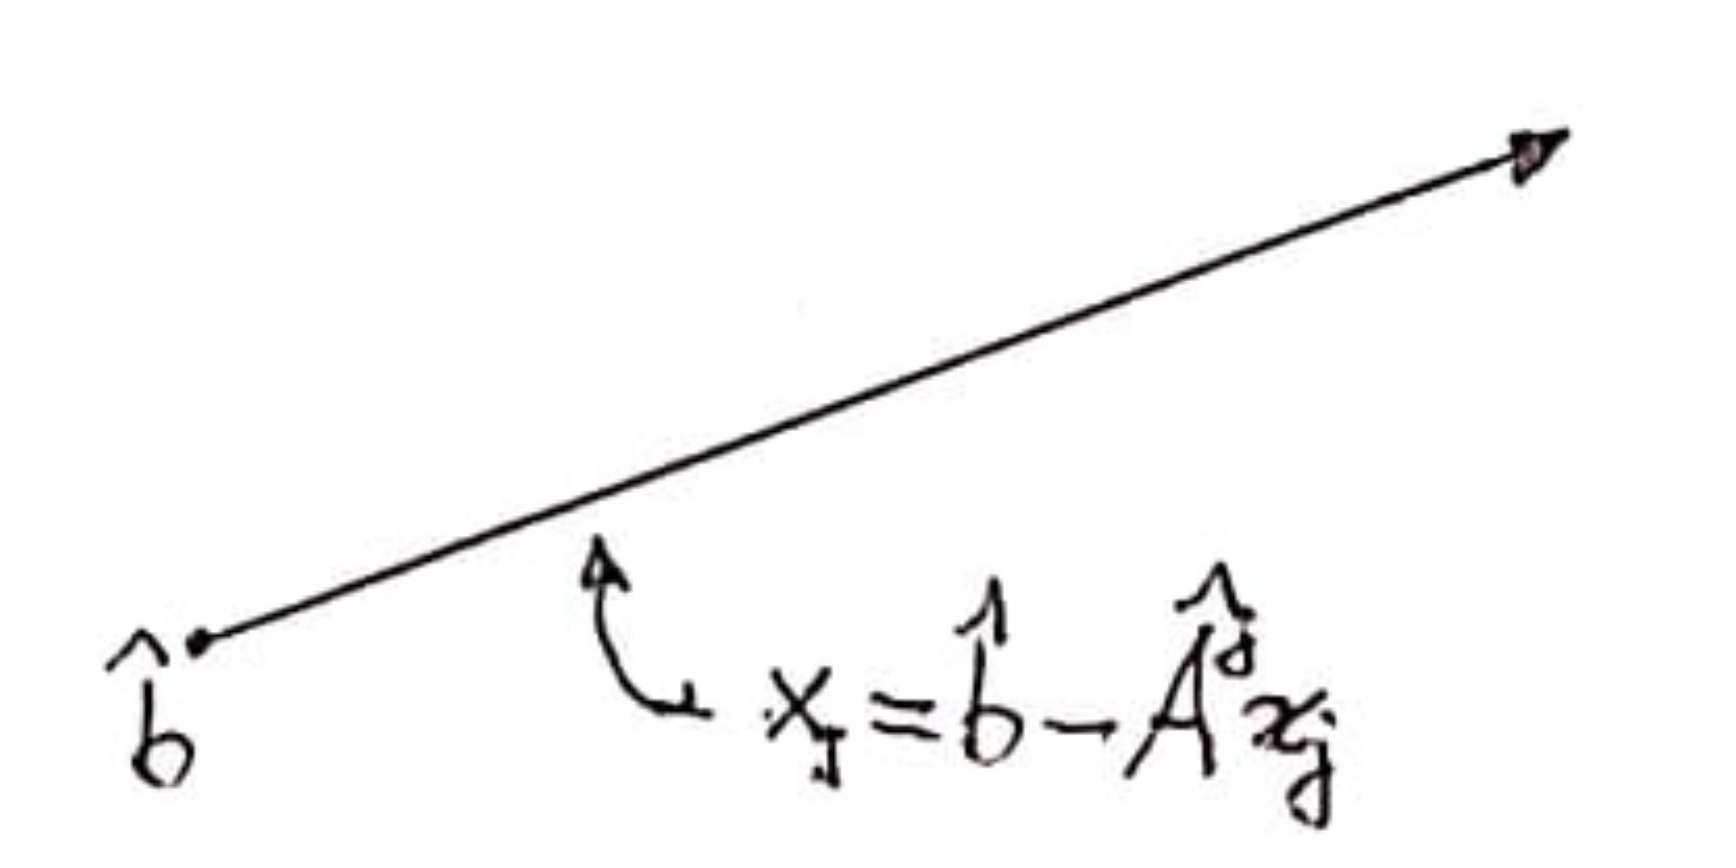
\includegraphics[width = 0.8\linewidth]{vetor.png}
  \caption{}
  \label{fig:vetor}
\end{figure}

\newpage

Mas, lembrando que se o conjunto das soluções $ Ax = b $, $ x \geq 0 $ é limitado,
não tem raio nem direção; tem arestas.
Se é ilimitado tem arestas que são raios.
Veja a Figura~\ref{fig:planos}.

\begin{figure}[!h]
  \centering
  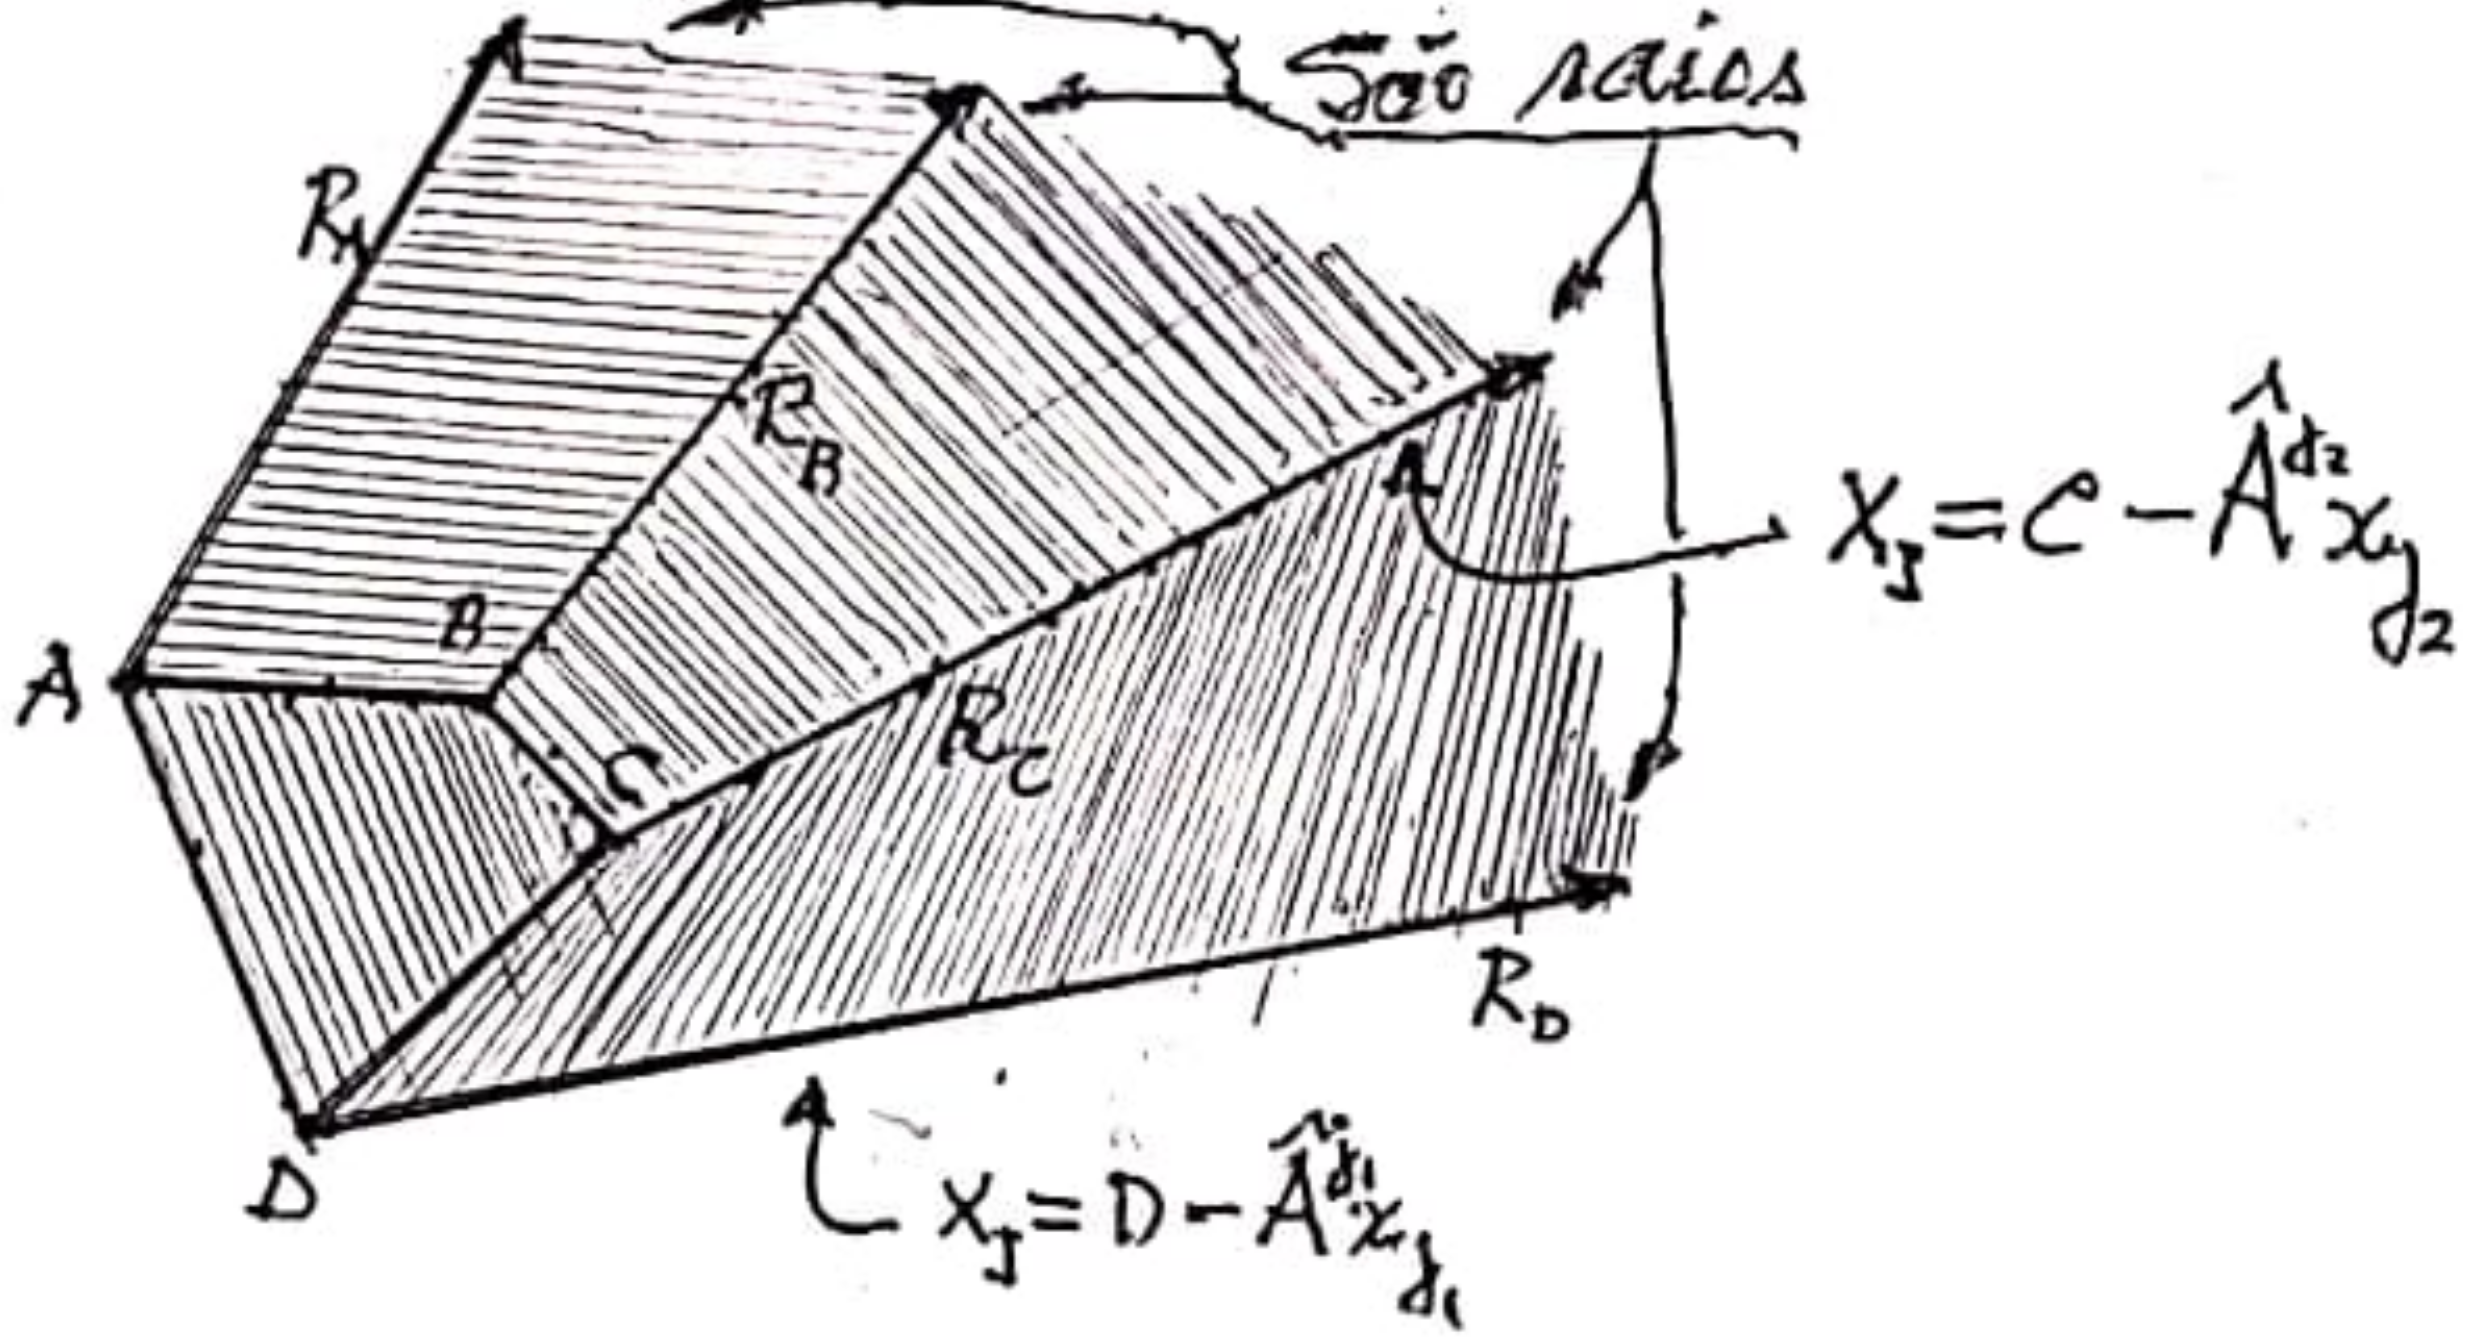
\includegraphics[width = \linewidth]{belo_desenho.png}  
  \caption{}
  \label{fig:planos}
\end{figure}

$ A, B, C \text{ e } D $ são pontos extremos, há oito arestas das quais quatro
são raios com origens em $ A, B, C \text{ e } D $.
Denominamos esses raios, respectivamente, por $ R_A, R_B, R_C \text{ e } R_D $.
O politopo é a interseção de cinco semiespaços, que são representados por cinco
inequações.
São elas:

\begin{enumerate}
  \item A que contém os pontos $ A $ e $ D $ e os pontos dos raios $ R_A $ e 
    $ R_D $.
    É a face invisível pela posição mostrada;
  \item A que contém os pontos $ A $ e $ B $ e os pontos dos raios $ R_A $ e
    $ R_B $;
  \item A que contém os pontos $ B $ e $ C $ e os pontos dos raios $ R_B $ e 
    $ R_C $;
  \item A que contém os pontos $ C $ e $ D $ e os pontos dos raios $ R_C $ e 
  $ R_D $;
  \item A que contém os pontos $ A, B, C \text{ e } D $.
\end{enumerate}

Cada inequação tem três variáveis, o que indica que após introduzir  as variáveis
de folga e de excesso obtém-se um sistema de cinco equações e oito variáveis.

Se, por exemplo, a solução atual for o ponto extremo $ C $, a variável candidata
para entrar na base seja $ x_j $ é $ \widehat{A}^j \leq 0 $, significa que ao
aumentar o valor de $ x_j $, nenhuma variável básica irá para zero.
As soluções vão percorrendo o raio $ R_C $.
Se algum $ \widehat{a}_{ij} > 0 $, então a solução percorrerá a aresta que vai
para $ B $ ou $ D $.

Se o conjunto das soluções de $ Ax = b $, $ x \geq 0 $ é \textbf{limitado}, este
não tem direção, logo, não tem raio.
Veja a Figura~\ref{fig:tetraedro}.

\begin{figure}[!h]
  \centering
  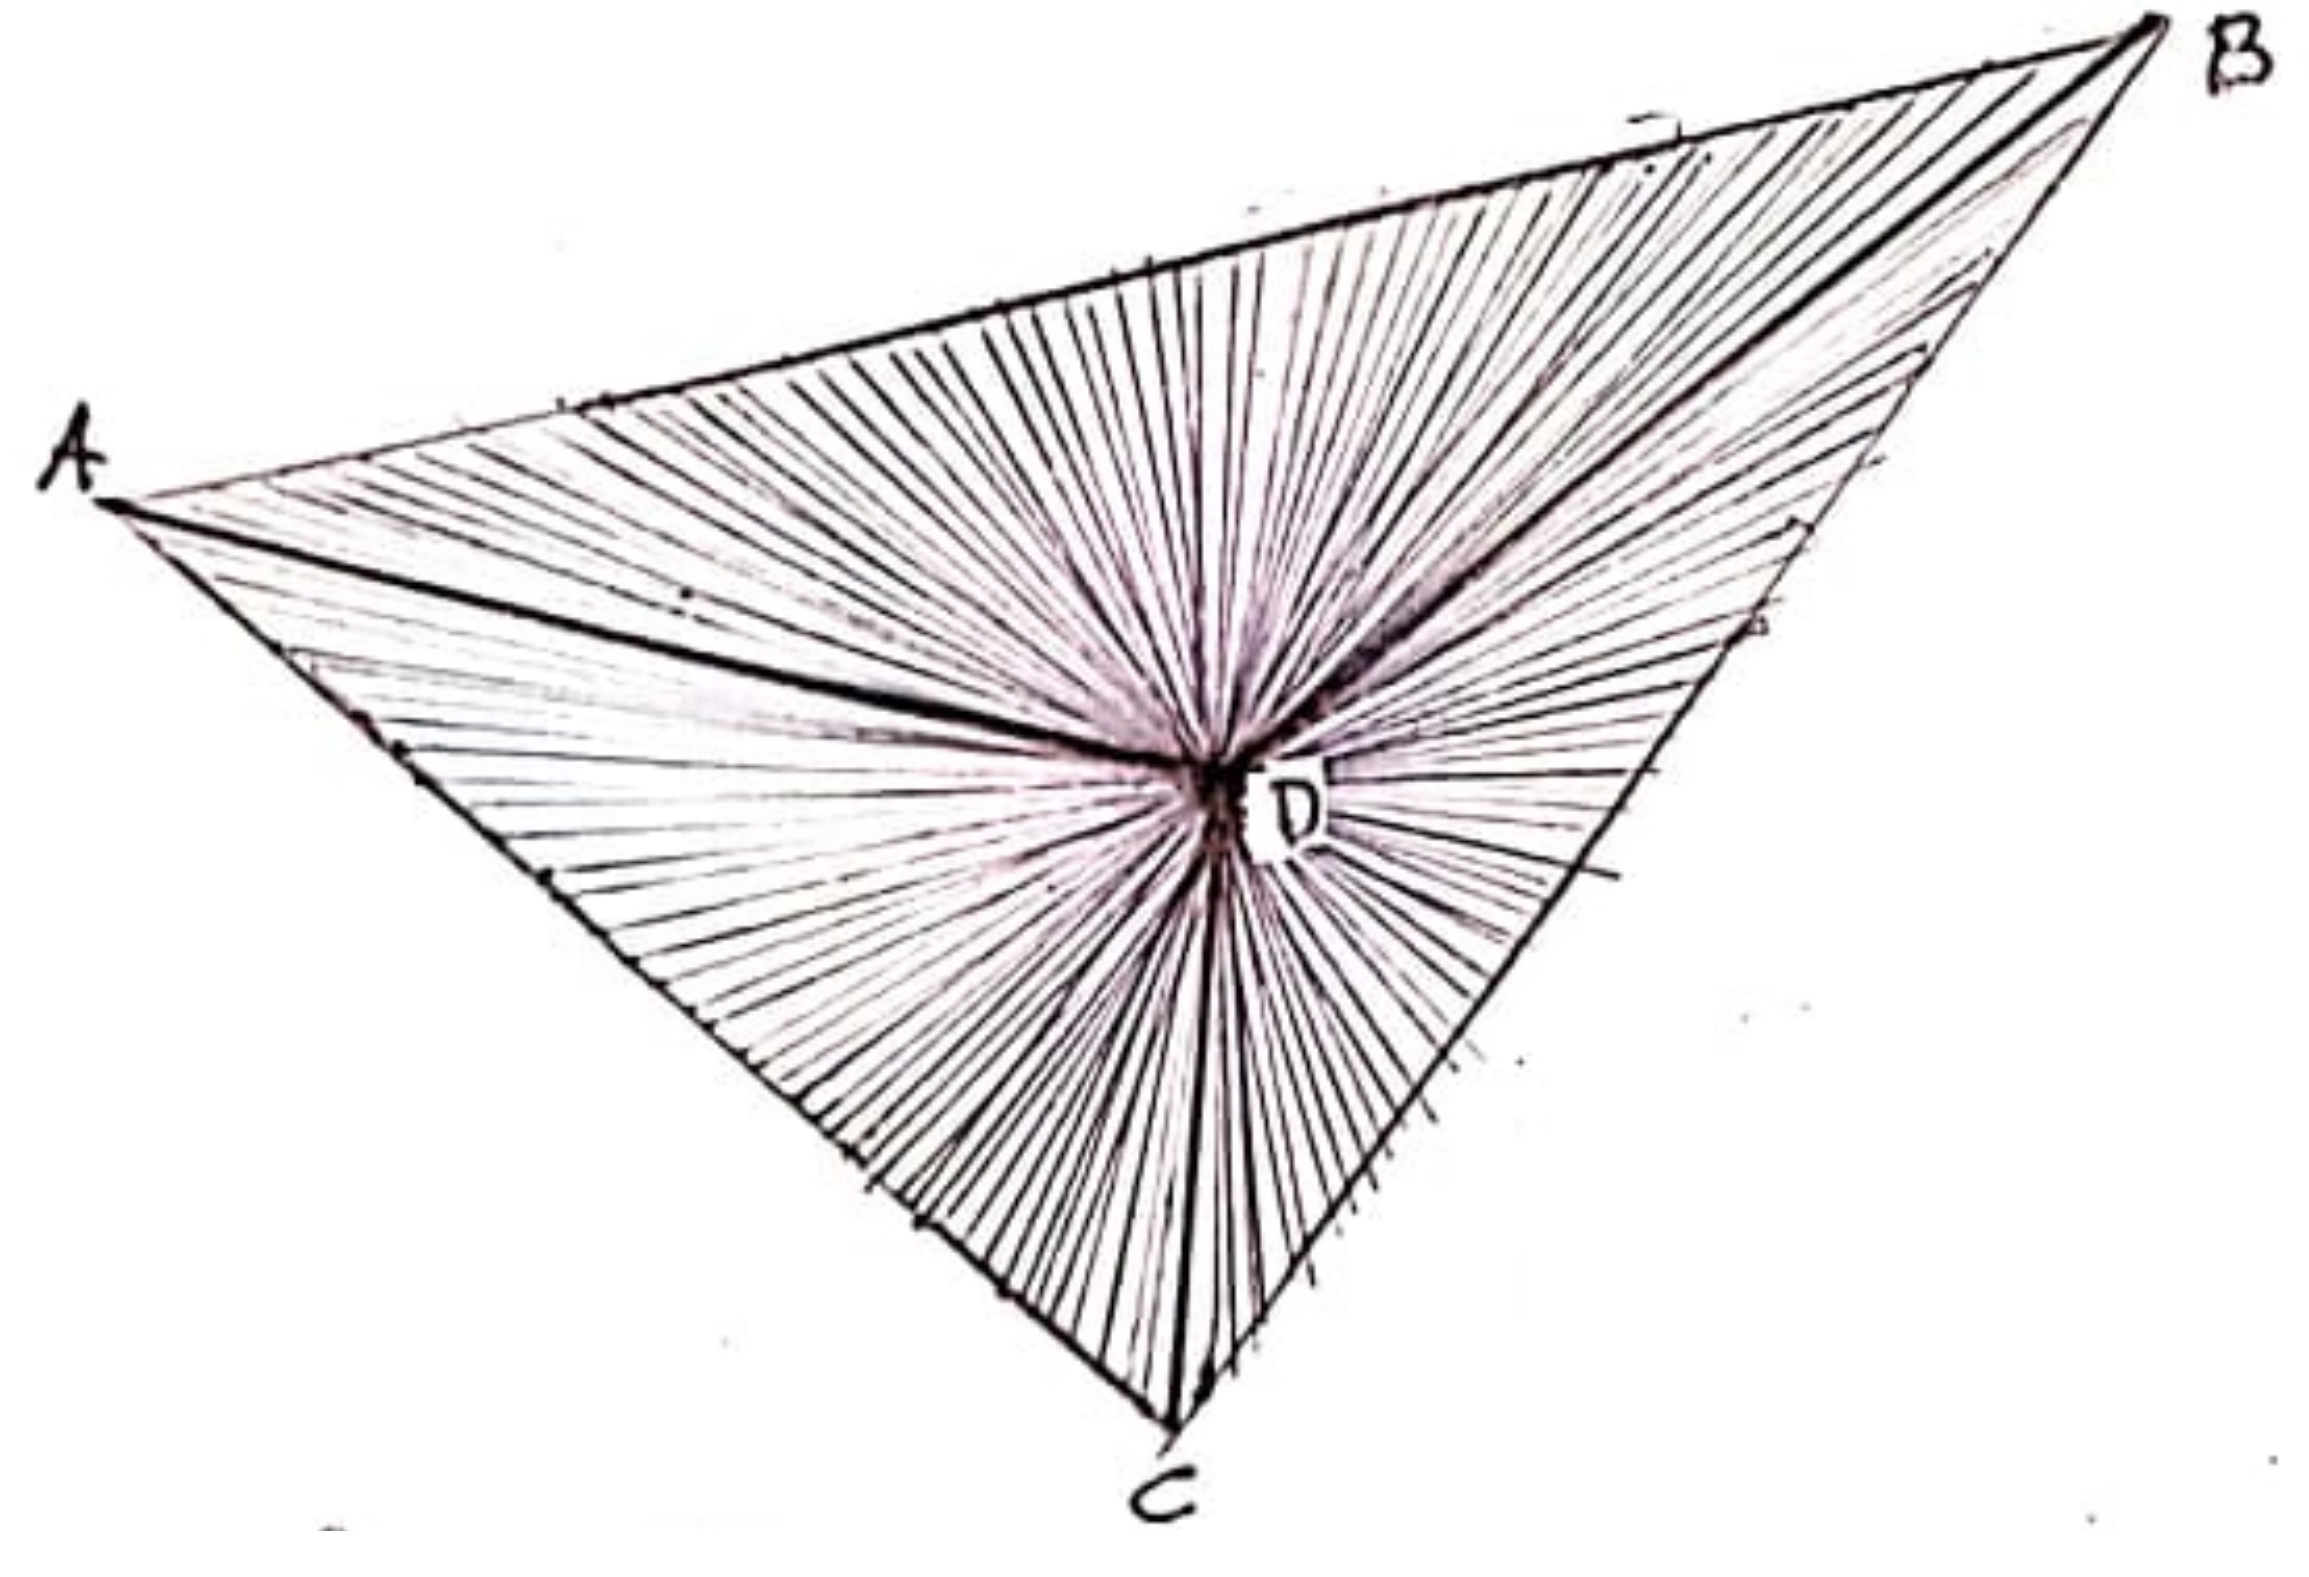
\includegraphics[width = 0.8\linewidth]{tetraedro.png}  
  \caption{Um tetraedro visto de cima}
  \label{fig:tetraedro}
\end{figure}

Os vértices $ A, B, C $ e $ D $ são pontos extremos.
Cada face correspondente a um plano e cada plano é definido pelos trios de pontos:
$ ABC, ABD, ACD \text{ e } BCD $.
O tetraedro é a interseção dos quatro semiespaços, em que pelo menos uma inequação
é do tipo "$ \geq $" e no máximo três.
A generalização para acontecer a Figura~\ref{fig:tetraedro} é:

\[
  \begin{cases}
    a_1x_1 + a_2x_2 + a_3x_3 &\leq \alpha_1 \\
    b_1x_1 + b_2x_2 + b_3x_3 &\stackrel[\leq]{\geq}{\phantom{=}} \alpha_2 \\
    c_1x_1 + c_2x_2 + c_3x_3 &\stackrel[\leq]{\geq}{\phantom{=}} \alpha_3 \\
    d_1x_1 + d_2x_2 + d_3x_3 &\leq \alpha_4 
  \end{cases}
\]

Note que esse politopo não tem direção.
Se $ d $ é um vetor não nulo e $ x_0 $ um ponto qualquer do politopo, para algum\\
$ \lambda > 0 $ o ponto $ x = x_0 + \lambda d $ não vai satisfazer o sistema  
acima.
Em outras palavras, o ponto $ x $ não pertencerá ao politopo.

Uma observação sobre os exemplos dados acima é que o espaço considerado é o 
$ \mathbb{R}^3 $.
As Figuras \ref{fig:planos} e \ref{fig:tetraedro} podem estar no espaço 
$ \mathbb{R}^{4} $, $ \mathbb{R}^{5} $, etc.
Como foi dito que eram resultados de interseção de inequações com três variáveis,
então poderiam estar no $ \mathbb{R}^{3}, \mathbb{R}^{4}, \mathbb{R}^{5} $, 
\ldots, qualquer um.
O número de variáveis diz qual é a dimensão \textit{mínima} do espaço em que 
essas inequações estão inseridas.
Então, ao ser apresentada uma equação ou uma inequação, deve ser dito em que 
espaço estão inseridas.
Por exemplo:

\begin{exemplo}
  O que representa a equação $ 2x - 5y = 7 $?
\end{exemplo}

Bem\ldots\ depende!
Se for em $ \mathbb{R}^{2} $ é uma \textit{reta}; se for em $ \mathbb{R}^{3} $ é
um \textit{plano}; e, se for em $ \mathbb{R}^{4} $, um \textit{hiperplano}.
A reta tem apenas uma dimensão, enquanto um plano tem duas.
O hiperplano depende da dimensão do espaço em que está inserido.
Por exemplo, a equação $ 3x + 2y - 5z + 7w = 4 $ não pode ser um plano.
Há aí, pelo menos, três variáveis livres, o que indica que representa um 
hiperplano de, pelo menos, três dimensões.
Por que "pelo menos"?
Se for em $ \mathbb{R}^{4} $, tem dimensão três, mas se for em $ \mathbb{R}^{5} $,
tem dimensão quatro.
O fato da quinta variável não aparecer na equação, diz que ela é uma variável 
livre.
A dimensão é o \textit{número de variáveis livres na equação}, logo, tem que se
dizer (dar) o espaço em que o objeto representado por aquela equação está 
inserido.

E qual a dimensão no caso de inequação?
Ganha mais uma dimensão, pois uma qualquer das variáveis não depende das outras.
Por exemplo, $ 2x + 3y \leq 6 $.
Se $ x = 1 $, $y$ não fica determinado. 
Há uma infinidade de valores que $ y $ pode assumir.
Isso independente de ser em $ \mathbb{R}^{2} $, $ \mathbb{R}^{2} $, \ldots.
Observe que $ 2x + 3y \leq 6 $ em $ \mathbb{R}^{2} $ é o semiespaço, isto é,
uma metade do plano $ \mathbb{R}^{2} $.
Qual é a dimensão?
Dois, é a resposta.

\begin{figure}[!h]
  \centering
  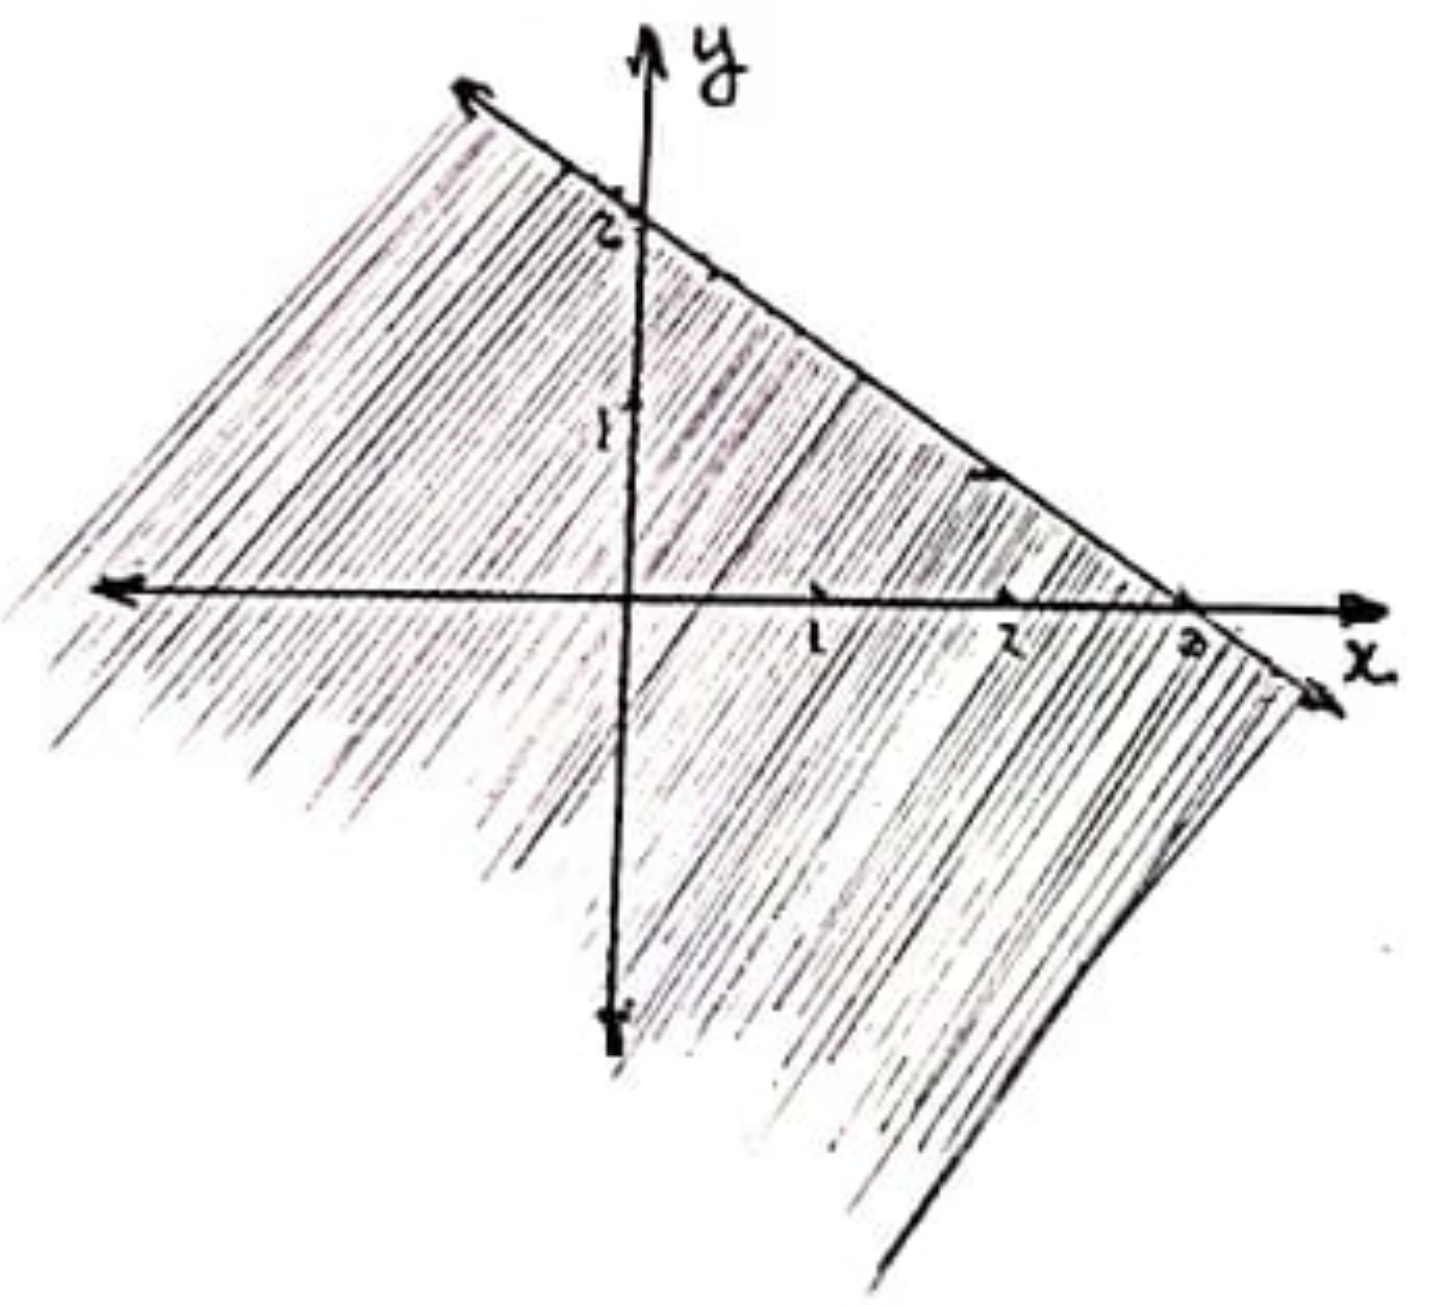
\includegraphics[width = 0.6\linewidth]{plano_simples.png}
  \caption{}
  \label{fig:planoSimples}
\end{figure}

Se $ 2x + 3y \leq 6 $ for em $ \mathbb{R}^{3} $.
A equação $ 2x +3y = 6 $ em $ \mathbb{R}^{3} $ é um plano.
Assim, $ 2x + 3y \leq 6 $ é um semiespaço formado pelo plano e mais os pontos
que estão de um lado do plano, logo, a dimensão do semiespaço é três.
%
%------------------------------------------------------------------------------
\end{document}
%==============================================================================
